\documentclass[12pt]{article}

\usepackage[a4paper,margin=1in]{geometry}
\usepackage{setspace}
\usepackage{mathptmx} % Times New Roman-like font
\usepackage{amsmath}
\usepackage{float}

\usepackage[style=apa, backend=biber]{biblatex}

\addbibresource{references.bib}

\usepackage{tikz}
\usetikzlibrary{shapes,arrows,positioning,fit,backgrounds,calc,decorations.pathreplacing}
\usepackage{svg}

\setlength{\parindent}{0pt}

\begin{document}

\begin{center}
\setstretch{1.3}

\vspace*{1cm}

{\LARGE \textbf{Asymmetric J-curve in Nepal's Pegged Exchange Rate Regime}} \\[4cm]

\vspace{0.5cm}
A thesis

\vspace{0.5cm}

Submitted to the 

\vspace{0.5cm}

Central Department of Economics

\vspace{0.5cm}

Faculty of Humanities and Social Sciences, Tribhuvan University 

\vspace{0.5cm}

In the Partial Fulfillment of the requirements for the Degree of

\vspace{0.5cm}

MASTER OF ARTS IN ECONOMICS

\vspace{1.5cm}

By:\\[0.5cm]
{\large Satish Chaudhary} \\[0.2cm]
TU Registration Number: 7-3-28-77-2016 \\[1.5cm]
Department of Economics \\[0.2cm]
Faculty of Humanities and Social Sciences \\[1.5cm]

Date of Submission: September 2026

\vspace*{1cm}

\end{center}

\newpage

% INTRODUCTION CENTERED
\begin{center}
\textbf{CHAPTER I}
\end{center}
\begin{center}
\textbf{INTRODUCTION}
\end{center}

\setstretch{1.5}

\vspace{0.5cm}

\noindent\textbf{1.1 Background of the Study}

The relationship between exchange rate fluctuations and its effect in trade flows is something economists have argued for decades, and still there is no clean answer. Many nations, including Nepal, adopted the strategy of currency devaluation to address the trade deficit after the collapse of Bretton Woods in early 1970s. The theoretical premise is that if your currency becomes cheaper, your export should look more attractive to foreign buyers while imports become more expensive for domestic consumers, and the trade balance should gradually improve. However, the real-world economy rarely works this way.

In the short term, trade volumes often remain stagnant due to rigidities such as existing contracts, shipping lags, and established consumer preferences. This phenomenon, where a devaluation initially exacerbates the trade deficit before eventually improving it, is conceptualized as the ``J-curve effect''. Early empirical failures to detect this effect were often rooted in the flawed assumption of symmetry—the belief that an economy responds identically to a 5\% appreciation as it does to a 5\% depreciation. Recent scholars have challenged this notion where \textcite{Shin2014-ap} introduced the Non-linear Autoregressive Distributed Lag (NARDL) model, providing a robust framework to analyze the asymmetric effects of currency movements. Utilizing this approach, \textcite{Nasir2021-xt} demonstrated that while depreciation generally benefits the US trade balance, appreciation detracts from it in a distinctly different manner. Similarly, \textcite{Arize2017-ar} found that trade flows in a sample of eight countries exhibited non-linear adjustments in most instances.

Within the South Asian context, the evidence is more ambiguous. \textcite{Bhat2021-ux} found that while India does not exhibit a conventional J-curve, depreciation has a more potent positive influence on the trade balance than appreciation has a negative one. Further complicating this, \textcite{Ganai2025-bv} argued that while depreciation provides long-term benefits, industrial capacity—rather than currency value alone—is the true driver of sustainable surpluses. Together, these studies suggest that exchange rate policy cannot be viewed as a standalone solution.

Furthermore, there is growing evidence that aggregate data often masks critical underlying patterns. \textcite{Bahmani-Oskooee2017-cf} illustrated that linear models applied to Singapore’s aggregate trade failed to capture relationships that became evident only through bilateral analysis. This was echoed by \textcite{Bahmani-Oskooee2019-ha}, who disaggregated US-China trade into 97 product categories and uncovered industry-level J-curves that were invisible in national totals. Similarly, \textcite{Bahmani-Oskooee2018-ij} found that currency fluctuations affect Japan-US trade variably depending on the commodity composition.

Nepal presents a particularly compelling anomaly in this literature. The country maintains a fixed bilateral peg to the Indian Rupee (NPR-INR), which consequently results in real effective exchange rate (REER) volatility against non-INR currencies driven by cross rate movements and inflation differentials. This creates a unique multilateral exchange rate dynamic. Most strikingly, Nepal defies standard economic intuition. Over the past two decades, the steady depreciation of the NPR against convertible currencies should, in theory, have narrowed the trade deficit; instead, the deficit has surged. This paradox exists because they relied on linear models that are incapable of capturing the asymmetric and ``messy'' reality of Nepal’s trade dynamics.

To understand what is driving this anomaly, if depreciation is failing to correct the deficit, the breakdown likely exists within the transmission mechanism. It is possible that Nepalese exporters lack the productive capacity to respond to price signals, or that the economy’s reliance on essential imports—such as fuel, food, and machinery—renders demand inelastic, meaning depreciation simply raises costs without reducing volumes. Alternatively, the divergent dynamics between the pegged Indian market and the floating global market may neutralize each other in aggregate data. Understanding why previous studies failed to resolve this paradox points directly to their reliance on linear models incapable of capturing these asymmetric realities. To address this, this study demonstrates how an advanced methodological approach can provide answers. By employing the Non-linear Autoregressive Distributed Lag (NARDL) approach, this study aims to determine whether the absence of a J-curve in Nepal is a result of model misspecification or a symptom of deep-seated structural failures within the economy.

\vspace{0.5cm}
\noindent\textbf{1.2 Statement of Problem}

For decades, Nepal has confronted a chronic trade deficit that has exhibited a persistent upward trajectory, defying the corrective mechanisms suggested by traditional economic theory. According to the standard orthodox view, currency depreciation should function as a natural stabilizer—enhancing the competitiveness of exports while discouraging the consumption of imports. However, Nepal presents a stark empirical paradox: despite the steady depreciation of the Nepalese Rupee (NPR) against the US Dollar over the past twenty years, the trade gap has not narrowed; rather, it has widened significantly.

This discrepancy is mirrored in the existing body of literature, where findings remain marked by significant divergence. While some scholars argue that exchange rate adjustments will eventually yield a correction, others contend that Nepal’s trade elasticities are too low to generate a meaningful impact. Much of this theoretical disagreement can be attributed to methodological limitations. By relying predominantly on linear models, previous research has operated under the assumption of symmetry—the notion that the economy responds to currency appreciation and depreciation in an identical, mirrored fashion. Such a simplification likely obscures the true, asymmetric dynamics of the Nepalese economy. Furthermore, by analysing the trade balance as a single aggregate metric, these studies frequently overlook the possibility that exports and imports respond to price signals through fundamentally different channels and time lines.

Compounding this complexity is Nepal’s unique monetary duality: a fixed peg with the Indian Rupee and a floating regime against other global currencies. There remains a critical scholarly void regarding whether the trade balance reacts differently to these two distinct regimes. The central mystery remains: why is devaluation failing to stabilize the deficit? Is this a failure of domestic supply capacity, a structural dependency on essential imports, or simply a failure of the linear models used to measure these effects? This study seeks to resolve this paradox by moving beyond linear assumptions and employing a non-linear framework to examine these asymmetries head-on.

\vspace{0.5cm}
\noindent\textbf{1.3 Research Questions}

The following research questions guide this study:

1. What is the nature of asymmetric J-curve effect in Nepal's aggregate trade balance?

2. How does Nepal’s trade balance respond asymmetrically to real currency appreciation versus real currency depreciation in the long-run?

3. How do the asymmetric J‑curve effects differ between Nepal's trade with India (fixed bilateral peg) and its trade with the Rest of the World (market‑determined REER)? 

\vspace{0.5cm}
\noindent\textbf{1.4 Objectives of Research}

The primary objective of this study is to evaluate the asymmetric and dynamic impact of real exchange rate fluctuations on Nepal's aggregate trade balance. To achieve this, the study pursues the following two specific objectives:

1. To examine the nature of the asymmetric J-curve effect in Nepal's aggregate trade balance/

2. To analyse the asymmetric response of Nepal's trade balance to real currency appreciation versus real currency depreciation in the long run.

3. To assess the asymmetric J‑curve effects differ between Nepal's  trade with India (pegged regime) and the Rest of the World (floating regime)


\vspace{0.5cm}
\noindent\textbf{1.5 Research Hypotheses}

\vspace{0.5cm}
\noindent\textbf{Hypothesis 1: Existence of the Asymmetric J-curve effect in Aggregate Trade}

This hypothesis tests whether real currency appreciation and depreciation exert statistically different effects on the trade balance in the long-run. 

\textbf{H\textsubscript{0}:} There is no asymmetric J-curve effect on Nepal's aggregate trade balance

\textbf{H\textsubscript{1}:} An asymmetric J-curve effect exists in Nepal's trade balance.

\vspace{0.5cm}
\noindent\textbf{Hypothesis 2: Asymmetric Adjustment to Appreciation versus Depreciation}

This hypothesis tests whether real currency appreciation and depreciation exert statistically different effects on the trade balance in the long-run. 

\textbf{H\textsubscript{0}:} The trade balance responds symmetrically to real appreciation and real depreciation in the long-run; the Wald test fails to reject $\theta^{+} = \theta^{-}$ in the NARDL long-run coefficients.

\textbf{H\textsubscript{1}:} The trade balance responds asymmetrically in the long-run; the Wald test rejects $\theta^{+} = -\theta^{-}$ at the 5\% significance level.

\vspace{0.5cm}
\noindent\textbf{Hypothesis 3: Regime dependent asymmetry}

This hypothesis tests whether the asymmetric response of the trade balance to real exchange rate movements differs between the India (pegged) and ROW (floating) segments of Nepal's trade.

\textbf{H\textsubscript{0}:} The asymmetric response of the trade balance to real exchange rate movements is identical for India and ROW trade; in particular, the long-run Wald test of symmetry yields the same outcome in both regimes.

\textbf{H\textsubscript{1}:} The asymmetric response differs between the India and ROW regimes.

\vspace{0.5cm}
\noindent\textbf{1.6 Limitations of Study}

While this research employs a sequential Linear ARDL–ECM–NARDL framework applied separately to aggregate, India, and ROW trade balances, certain inherent limitations in the data and economic context must be acknowledged.

First, due to the availability of consistent long-term records, this study utilizes annual rather than quarterly data over the 45-year sample period (1980-2024). While annual data provides a robust historical perspective, it may smooth over very short-term fluctuations and blend the initial deterioration and recovery phases of J-curve into a single observation. Consequently, the short run effects should be interpreted as year one impacts rather than quarter-by-quarter adjustments. This was a necessary trade off to ensure the consistency across all variables. 

Second, the sample period encompasses significant exogenous shocks, most notably the 1990 trade liberalization, the 2008–2009 global financial crisis, the 2015 Gorkha Earthquake, and the COVID-19 pandemic. Such events can introduce structural breaks that may exert non-linear effects on trade volumes. To mitigate this, the study employs CUSUM and CUSUMSQ tests to evaluate parameter stability, ensuring that the estimated coefficients remain reliable despite these disruptions.

Third, Nepal receives substantial worker remittances, equivalent to approximately 25\% of GDP, which significantly affect the current account and import capacity. These inflows may interact with exchange rate dynamics by sustaining import demand regardless of currency movements, potentially bias the long-run exchange rate coefficients. While remittance data is available, incorporating it as an additional regressor falls outside the scope of this study and represents a potential direction for future research.

A further limitation concerns the exchange rate measure used for the India-specific model. The study employs the multilateral REER for both India and ROW analyses. While REER is appropriate for aggregate and ROW trade, a bilateral real exchange rate (NPR/INR adjusted for inflation) would be more accurate for the India model. However, consistent data for such a bilateral series over 1980–2024 is not readily available. Future research could construct this series and compare results.

Finally, a methodological limitation arises from the lag structure selected by the information criteria (AIC;SIC), which chose lag-0 both the positive and negative partial sums across all three trade balance regimes. Under this parsimonious specification, the short run asymmetry cannot be formally tested; therefore, the present study tests long run symmetry only. This approach is consistent with the original \textcite{Shin2014-ap} formulation and is justified by the degree of freedom constraint imposed by the sample size ($T \approx 43$), as well as the economic reality that Nepal's de facto peg to the Indian rupee mutes short run transmission. Future research with a longer sample could visit short-run asymmetry once additional annual observations are available.


\vspace{0.5cm}
\noindent\textbf{1.7 Organization of Study}

The study is organized into five chapters. The first chapter serves as the introduction and encompasses the background of the study, statement of the problem, objectives, hypothesis formulation, limitations, and the structure of the study. The second chapter presents a review of the literature, including both theoretical and empirical reviews, and identifies the research gap. The third chapter describes the research methodology, covering the research design, nature and scope of data, tools and techniques of data collection, and model specification. The fourth chapter is devoted to data analysis and presentation. Finally, the fifth chapter provides the summary, conclusions, and recommendations arising from the research.

\newpage
\begin{center}
\textbf{CHAPTER II}
\end{center}
\begin{center}
\textbf{REVIEW OF LITERATURE}
\end{center}

The relationship between exchange rate fluctuations and the trade balance has remained one of the most contentious subjects in international economics for nearly seven decades. Central to this discourse is the J-Curve phenomenon—a theoretical construct suggesting that currency devaluation or depreciation may initially exacerbate a trade deficit before eventually improving it. This counter intuitive pattern carries profound implications for macroeconomic management, particularly for developing economies like Nepal, which grapple with persistent trade imbalances and a constrained set of policy instruments. Determining whether the J-Curve operates within the Nepalese context is more than an academic exercise; it is a critical inquiry into whether currency devaluation can serve as a viable policy tool to alleviate the country's chronic trade deficit \parencite{Bahmani-Oskooee_2004-hu}. In the specific context of Nepal, \textcite{chaulagai2015} explicitly notes that investigating the existence of the J-curve phenomenon in the country's foreign trade sector holds substantial practical relevance for evaluating whether exchange rate depreciation can be employed as an effective instrument to correct the nation's presistent external imbalances. 

This chapter provides a comprehensive review of the existing literature to establish the conceptual and empirical foundation of this study. The review is structured to build a rigorous theoretical base while systematically identifying the scholarly voids that justify this investigation. The chapter begins by examining the theoretical underpinnings of the trade-exchange rate relationship, starting with the Marshall-Lerner condition. This section provides the analytical and mathematical basis for understanding how exchange rate transmissions affect trade balances. This is followed by an analysis of the J-Curve phenomenon, tracing its evolution from \textcite{Magee1973-dr} original formulation to the operational definitions used in contemporary econometrics. The theoretical discussion concludes by exploring the existence of asymmetric effects—a critical insight that provides the primary motivation for employing the Nonlinear Autoregressive Distributed Lag (NARDL) methodology.

The second section surveys the global empirical landscape, reviewing foundational studies from the 1980s and 1990s, as well as more recent bilateral and regional analyses. Particular attention is paid to the methodologies employed and the limitations of previous findings. \textcite{Bahmani-Oskooee1985-jx} was among the pioneers to empirically test the J-curve  hypothesis using standard econometric techniques. In their comprehensive surveys, \textcite{Bahmani-Oskooee_2004-hu} and \textcite{Bahmani-Oskooee2010-bs} systematically reviewed a vast array of empirical contributions across different countries and time periods. Their synthesis indicates that the evidence regarding the J-Curve remains highly mixed; while a substantial number of studies find supporting evidence, the results are notably sensitive to the choice of empirical methodology, data frequency, model specification, and the specific sample periods under investigation. This inherent uncertainty underscores the importance of continuously revisiting the question with more advanced estimation techniques.

The third section is dedicated to a rigorous review of NARDL literature, detailing its theoretical development, mathematical specification, and its successful application in J-Curve studies worldwide. The NARDL framework, formally developed by \textcite{Shin2014-ap}, offers a significant methodological advancement by allowing for the decomposition of exchange rate movements into positive (appreciation) and negative (depreciation) partial sums, thereby capturing their differential impacts on the trade balance.

The fourth section narrows the focus to South Asian and Nepal-specific evidence, critically evaluating the work of scholars such as \textcite{chaulagai2015}, \textcite{Bishwakarma2024-fa}, \textcite{pathak2020}, and \textcite{Adhikari2020-rr}. By synthesizing these findings, this section explicitly articulates the research gap that the present study seeks to address. The chapter concludes by establishing the methodological framework for the investigation and aligning the research contribution with the overarching study objectives.

\vspace{0.5cm}
\noindent\textbf{2.1 Theoretical Foundations}

The foundational framework for modelling the relationship between exchange rates, income, and the trade balance is the imperfect substitutes model, comprehensively formalized in the seminal work of \textcite{Goldstein1985}. This model departs from the classical assumption that goods across borders are perfectly interchangeable, positing instead that domestic and foreign goods are imperfect substitutes. Consequently, the demand for a nation's imports and exports is driven by two primary macroeconomic forces: relative prices (captured by the real exchange rate) and the purchasing power of consumers (captured by domestic and foreign incomes). According to this framework, a country's import demand function is expressed as $M = f(Y, P_m/P_d)$, where $Y$ represents domestic income and $P_m/P_d$ represents the relative price of imports to domestic goods. Conversely, the export demand function is defined as $X = f(Y^*, P_x/P_f)$, where $Y^*$ is foreign income and $P_x/P_f$ is the relative price of exports to foreign goods. Aggregating these demand functions reveals that the trade balance is fundamentally determined by domestic income, foreign income, and the real exchange rate: $TB = f(Y, Y^*, REER)$. This theoretical specification is critical for empirical modelling. It dictates that any rigorous econometric analysis of the trade balance must control for both domestic and foreign income to isolate the pure price effects of exchange rate fluctuations. If foreign income ($Y^*$) is omitted, the model suffers from omitted variable bias, as shifts in global or bilateral demand could be erroneously attributed to exchange rate movements. Therefore, the imperfect substitutes model provides the direct theoretical justification for the inclusion of Nepal's real GDP as a domestic-income control in the ARDL and NARDL specifications employed in this study; the foreign-income channel is treated in the pilot-estimation stage and then excluded from the final specification on parsimony grounds.

While the imperfect substitutes model establishes the variables that drive trade flows, it is the price elasticities embedded within these demand functions that determine the direction of the trade balance response to currency devaluation. This brings us to the Marshall-Lerner condition, the foundational analytical framework for understanding the transmission of exchange rate fluctuations to trade balances. While the conceptual seeds were planted by Marshall in his discourse on money, credit, and commerce, it was Lerner who provided the formalized mathematical expression that remains the cornerstone of international trade theory. The Marshall-Lerner condition posits that a devaluation of the domestic currency will improve the trade balance in long run, under constant terms of trade, if sum of the absolute values of the price elasticities of demand for exports and imports is greater than one. To appreciate the policy implications of this condition, one must consider the inherent tension between price and volume effects. For instance, if a country devalues its currency by 10\%, its exports become cheaper for foreign buyers, while imports become more expensive for domestic consumers. Theoretically, this should trigger an increase in export volumes and a decrease in import volumes. However, the ML condition suggests that these volume responses must be sufficiently elastic to outweigh the immediate negative impact of higher import prices. This is expressed mathematically as $|\eta_x| + |\eta_m| > 1$  where $\eta_x$ and $\eta_m$ represent the price elasticities of export and import demand, respectively. When this condition is satisfied, the volumeigi effect dominates, and the trade balance improves. Conversely, if demand is relatively inelastic—as is common in developing economies for essential goods—the devaluation may actually exacerbate the trade deficit by increasing the cost of imports without inducing a significant reduction in volume \parencite{Bahmani-Oskooee_2004-hu}.

A pivotal refinement to this theory was provided by \textcite{Rose1989-bs}, who demonstrated that the Marshall-Lerner condition is a necessary but not sufficient requirement for short-run trade balance improvement. Their research revealed that even when the elasticity condition is met, trade balances may initially deteriorate due to adjustment lags—such as existing contracts and shipping delays. This finding provided the theoretical bridge to the J-Curve phenomenon, suggesting that the perceived contradiction between ML theory and empirical reality is often a matter of timing rather than a fundamental failure of the theory. \textcite{Rose1989-bs} emphasized that the distinction between short-run contraction and long-run expansion is critical to understanding exchange rate pass-through, and he established explicit hypothesis tests to distinguish between these time-bound effects. His work provided a rigorous econometric framework for testing the J-Curve hypothesis, moving it from a descriptive narrative to a testable statistical proposition.


For a developing, landlocked economy like Nepal, these theoretical considerations are not merely academic—they are central to the country's economic vulnerability. Nepal's reliance on essential imports, such as petroleum, pharmaceuticals, and machinery, suggests a high degree of import in-elasticity. In such a scenario, the Marshall-Lerner condition may not hold; depreciation simply raises the domestic cost of survival without fostering domestic substitution. This structural reality is echoed in the work of \textcite{pathak2020}, whose elasticity estimates provide the empirical context for why the ML condition may be elusive in Nepal. This theoretical tension helps explain the findings of \textcite{chaulagai2015}, who observed an absence of J-Curve effects, suggesting that Nepal's trade dynamics may be governed more by structural rigidities than by currency fluctuations.

The formal conceptualization of the J-Curve phenomenon is widely attributed to \textcite{Magee1973-dr}, who recognized that the timing of trade contracts fundamentally dictates how exchange rate fluctuations transmit to the trade balance. Magee's primary contribution was the identification of "adjustment lags"; because international trade contracts are often denominated in foreign currencies and renegotiated infrequently, the effects of devaluation are not instantaneous. Following a devaluation, existing import contracts—signed at previous rates—continue to be executed, causing the cost of imports to rise immediately in domestic terms. In contrast, the benefits of increased export competitiveness take longer to materialize as new contracts must be negotiated and signed at the new, more favourable prices. This temporal mismatch creates the characteristic J-shaped trajectory: an initial deterioration of the trade balance, followed by a gradual improvement as volume effects eventually dominate price effects.

In contemporary econometric research, the operational definition of the J-Curve has evolved from \textcite{Magee1973-dr}'s original narrative into a testable statistical hypothesis. \textcite{Bahmani-Oskooee1985-jx} provided the empirical framework that guides most modern studies: the J-Curve is present if the trade balance exhibits a negative (deteriorating) relationship with the exchange rate in the short run, while maintaining a positive (improving) relationship in the long run. In practice, this is tested by examining the signs and significance of coefficients within Error Correction Models (ECM) or Non-linear Autoregressive Distributed Lag (NARDL) models. A J-Curve is confirmed when the short-run coefficient for depreciation is negative and significant, while the long-run coefficient is positive and significant. This framework was further refined by \textcite{Rose1989-bs}, who established explicit hypothesis tests to distinguish between these time-bound effects.

\vspace{0.5cm}
\noindent\textbf{2.2 Beyond Symmetry: The Case for Asymmetric Effects}

Traditional econometric frameworks analysing the relationship between exchange rates and trade balances have long operated under the assumption of symmetry—the notion that currency appreciation and depreciation exert equal but opposite pressures on the trade balance. This assumption was fundamentally embedded in linear models, which employed a single exchange rate coefficient to capture the aggregate relationship. However, this orthodox approach has been increasingly contested in recent literature, giving rise to non-linear and asymmetric models that allow for differential effects based on the direction of the currency movement \parencite{Shin2014-ap, Bahmani-Oskooee2015-ev}.

The theoretical justification for asymmetry is rooted in several systemic economic frictions. First, import demand in developing economies is frequently characterized by high levels of inelasticity, particularly regarding essential commodities. When a currency depreciates, the prices of critical imports—such as pharmaceuticals, petroleum, and industrial machinery—rise. However, because these goods are essential for survival and production, import volumes do not decline proportionally. Conversely, during currency appreciation, the fall in import prices may not trigger a corresponding increase in volume, as domestic demand for these essentials is already saturated. This creates a directional asymmetry that linear models, by their very nature, are unable to capture. Second, the composition of trade often differs fundamentally between exports and imports; developing nations frequently export primary commodities (which may have higher elasticity) while importing manufactured goods (which are often inelastic). Third, market structures, particularly in oligopolistic industries, often lead to "sticky" pricing, where firms are quicker to raise prices during depreciation to protect margins than to lower them during appreciation. Finally, government interventions—including tariffs and quotas—introduce non-linearities that vary significantly depending on whether the currency is rising or falling \parencite{Goldstein1985, Bahmani-Oskooee_2004-hu, pathak2020}.

The empirical catalyst for this shift was provided by \textcite{Bahmani-Oskooee2015-ev}, whose research fundamentally transformed J-Curve analysis. Their work demonstrated that the symmetry assumption in linear models was overly restrictive and often masked critical non-linear dynamics. By decomposing exchange rate changes into positive (appreciation) and negative (depreciation) components, they revealed that the effects on trade balances often differed not only in magnitude but occasionally in sign. Their findings suggested that linear models, by imposing symmetry, risked producing misleading conclusions regarding the existence and nature of the J-Curve. This methodological insight provides the direct impetus for the present study application of the Nonlinear Autoregressive Distributed Lag (NARDL) framework.

The policy implications of this asymmetry are particularly acute for Nepal. If exchange rate movements are asymmetric, policy-makers cannot assume that a devaluation will mirror the effects of an appreciation. Given Nepal's structural reliance on essential imports, it is highly probable that depreciation worsens the trade balance more than appreciation improves it. In such a scenario, currency devaluation becomes a far less effective tool for deficit correction than symmetric models would suggest. Consequently, the adoption of the NARDL methodology is essential to uncover these asymmetric transmissions and provide a more accurate diagnostic of Nepal's trade dynamics \parencite{chaulagai2015, Bishwakarma2024-fa, pathak2020}.

\vspace{0.5cm}
\noindent\textbf{2.3 Global Empirical Evidence}

The empirical investigation of the J-Curve has produced a substantial body of literature spanning nearly four decades, with hundreds of studies published across leading journals in international economics. The earliest empirical studies established the basic methodological approaches and documented the phenomenon across different country groups, while subsequent studies refined the methodology and expanded the geographical and temporal coverage to include developing countries, emerging markets, and transition economies. This section provides an incredibly detailed review of the foundational empirical literature that established the research agenda for J-Curve studies, with attention to both findings and methodological innovations \parencite{Bahmani-Oskooee1985-jx, Bahmani-Oskooee_2004-hu, Bahmani-Oskooee2010-bs}.

\textcite{Gylfason1984-ys} examined whether devaluation improved the current account and found that the effects varied based fundamentally on the Marshall-Lerner condition's validity, publishing in the European Economic Review. Their work was among the first to explicitly link the theoretical Marshall-Lerner condition to empirical testing in a systematic way. The authors noted that the success of devaluation as a policy tool depended critically on the trade elasticities, which varied significantly across countries and over time. This study established the critical link between theory and empiric that has characterized subsequent J-Curve research.

\textcite{Bahmani-Oskooee1985-jx} conducted one of the earliest and most influential comprehensive empirical investigations of the J-Curve phenomenon in Less Developed Countries, publishing in the Review of Economics and Statistics, one of the discipline's premier journals. Using quarterly data from multiple developing economies, they tested whether trade balances initially deteriorated following currency devaluation before showing improvement in subsequent quarters—the defining characteristic of the J-Curve. The methodology involved estimating error correction models and examining the sign and significance of both short-run and long-run coefficients to determine whether the J-Curve pattern was present. The findings provided evidence supporting the J-Curve in several LDCs, particularly those with more flexible exchange rate regimes. Importantly, the study established the empirical framework—the error correction model with separate short-run and long-run coefficients—that subsequent researchers would adopt and refine over the subsequent four decades. The study also highlighted the critical importance of distinguishing between the short-run and long-run effects, a methodological innovation that has guided much subsequent research.

\textcite{Rose1989-bs} made a crucial contribution by providing a precise definition of the J-Curve and testing it using aggregate data from both industrial and developing countries, published in the Journal of Monetary Economics. Their methodology involved testing whether trade balance and real exchange rate were co-integrated and whether the short-run and long-run coefficients had the expected signs. Rather than finding the straightforward J-Curve pattern in all cases, they found an "S-shaped" curve in some cases—a pattern where the trade balance initially improves rather than deteriorates, then deteriorates, and then improves again in a more complex pattern. This finding significantly complicated the simple J-Curve narrative and suggested that the relationship between exchange rate and trade balance might be far more complex than initially thought. Their study emphasized that the J-Curve was not a universal phenomenon and that country-specific factors played a crucial role in determining whether and how it manifested.

Early challenges to the universality of the J-Curve were noted by \textcite{Rose1989-bs}, whose cross-country analysis of developing economies revealed that the phenomenon is remarkably fragile. Rose demonstrated that empirical results are highly sensitive to the choice of exchange rate measures and the specific time periods analysed, concluding that the Marshall-Lerner condition does not hold universally. This suggested that country-specific structural factors are not merely secondary variables but are decisive in determining trade responses. The utility of this disaggregated approach was further validated by Bahmani-Oskooee and Brooks (1999), who analysed bilateral J-Curves between the United States and its various trading partners. Their findings revealed significant heterogeneity; while some partners exhibited a classic J-Curve, others showed no such effect. 

\textcite{Bahmani-Oskooee1991-or} extended the earlier work in a significant way by examining the long-run relationship between trade balance and real effective exchange rate using co-integration techniques that were at the cutting edge of econometric methodology at the time. This study was important because it introduced the concept of co-integration to J-Curve analysis—a methodological advancement that allowed researchers to test for long-run equilibrium relationships while accounting for short-run dynamics in a unified framework. The findings suggested a long-run equilibrium relationship in many cases, but the short-run dynamics varied significantly across countries in important ways that had policy implications. This study highlighted the essential importance of treating short-run and long-run effects separately and established the co-integration framework that would become standard in subsequent J-Curve studies.

The influence of external shocks and economic transitions further complicates the J-Curve narrative. \textcite{Lal2002-ca} examined East Asian economies during the Asian financial crisis, finding mixed evidence that highlighted the role of exchange rate regimes and structural constraints. Similarly, \textcite{Grigoryan2015-gz} analyzed Armenia's transition economy, finding that the J-Curve operated in the short run but lacked long-term consistency. These studies suggest that for small, open, or transitioning economies, the J-Curve is not a static law but a dynamic response shaped by the economic environment.

Moving beyond bilateral partners, research has also explored sectoral asymmetries. \textcite{Bahmani-Oskooee2009-gm} extended this logic to the industry level, analyzing Sweden-United States trade. Their ground-breaking study revealed that J-Curve effects vary fundamentally across different product categories, with some industries showing clear J-curves while others exhibited reverse patterns. This evidence is particularly relevant for the current study, as it suggests that the trade balance of a country like Nepal may be driven by specific commodity groups rather than a uniform national response.

Finally, a meta-analysis by \textcite{Kallianiotis2022-po} synthesized decades of research, concluding that while the theoretical foundation of the J-Curve remains robust, the empirical evidence is characterized by significant variation. This synthesis confirms that the inconsistency in previous findings is likely a product of differing methodological approaches and country-specific contexts, providing a strong justification for the tailored, non-linear approach adopted in this research.

\vspace{0.5cm}
\noindent\textbf{2.4 The NARDL Methodology: Development and Applications}

The emergence of the Nonlinear Autoregressive Distributed Lag (NARDL) methodology represents a pivotal advancement in J-Curve research, fundamentally altering the analysis of exchange rate-trade balance transmissions. Developed by \textcite{Shin2014-ap}, the NARDL framework extends the linear ARDL bounds testing approach pioneered by \textcite{Pesaran2001-kt} to accommodate asymmetric effects within a rigorous econometric structure. This section examines the development of the NARDL model and its application to J-Curve studies, highlighting its theoretical and empirical superiority over traditional linear frameworks.

The foundation of this approach lies in the linear ARDL model introduced by \textcite{Pesaran2001-kt}. This framework revolutionized co-integration analysis by permitting the inclusion of variables with differing orders of integration—specifically a mix of I(0) and I(1) variables—within a single coherent  model. Unlike the Johansen co-integration method, which necessitates that all variables be integrated of the same order, the ARDL approach is particularly robust for small sample sizes and provides reliable inference even when integration orders are mixed or unknown. By comparing the F-statistic against critical value bounds, researchers can determine the existence of a long-run relationship without the need for exhaustive pre-testing of unit roots, making it an ideal tool for analysing the often-volatile trade data of developing economies.

Building upon this foundation, \textcite{Shin2014-ap} introduced a non-linear extension that allows for the decomposition of explanatory variables into asymmetric components. The core methodological innovation involves partitioning a variable—such as the exchange rate ($X_t$)—into positive and negative partial sums. Specifically, $X_t^{+} = \sum_{i=1}^{t} \max(\Delta X_i, 0)$, representing cumulative appreciation, and $X_t^{-} = \sum_{i=1}^{t} \min(\Delta X_i, 0)$, representing cumulative depreciation. This decomposition enables the model to capture three distinct types of asymmetry: asymmetric long-run effects where the coefficients differ $\beta^{+} \neq \beta^{-}$ asymmetric short-run adjustment speeds, and asymmetric dynamic multipliers, which map the divergent adjustment paths following positive and negative exchange rate shocks. A defining feature of the NARDL specification—emphasised by \textcite{Shin2014-ap} themselves—is that the partial-sum processes and the level variables are permitted to carry different lag orders within a single regression. This property, which is the framework's "crucial feature," explicitly accommodates the empirical regularity that the optimal lag length of the partial sums often differs from the optimal lag length of the dependent variable and the level regressor. Consequently, the data-driven selection of lag-0 on the partial sums (when information criteria so indicate) is a legitimate outcome of the model, not a violation of its structure, and aligns with the parsimony principle embedded in the underlying ARDL bounds-testing approach.

The NARDL specification offers four critical advantages over its linear predecessors. First, it facilitates the direct testing of asymmetry through Wald tests on coefficient restrictions, providing a statistically rigorous basis for rejecting the symmetry hypothesis. Second, by producing separate estimates for appreciation and depreciation, it allows for more nuanced and targeted policy prescriptions. Third, it can uncover J-Curve effects that remain latent in linear models due to the "averaging" of opposing forces. Finally, the use of dynamic multipliers provides a visual and quantitative representation of how the trade balance evolves over time, offering a far more sophisticated diagnostic of the economy's response to currency volatility than a single coefficient ever could \parencite{Shin2014-ap}.

The small-sample efficiency of the NARDL framework is particularly well established in the recent applied literature. \textcite{Abegaz2024-wp}, in a NARDL analysis of Ethiopia's trade balance over 1992--2022 ($T = 31$), explicitly justifies the use of the framework on grounds that it "provides efficient and reliable estimates in case of low and limited samples" and "allows the variables to be integrated with different orders of integration, and estimated at different lag lengths in one regression model." \textcite{Iqbal2021-pu} document a similar pattern in bilateral NARDL applications to Pakistan's trade with eight partners, and the J-Curve applications surveyed in \textcite{Bahmani-Oskooee2016-xv} routinely report lag orders on the partial sums that differ from those on the level terms. These precedents indicate that the NARDL framework is the method of choice when the available sample cannot support a heavily parametrised specification, and they provide direct support for the present study's small-sample context ($T \approx 43$).

The transition from theoretical framework to empirical application was most prominently exemplified by \textcite{Bahmani-Oskooee2016-xv}, who published a seminal application of the NARDL approach to J-Curve analysis in the Open Economies Review. By analysing bilateral trade data between the United States and four major partners—Canada, China, Japan, and Korea—their research provided a definitive empirical case for asymmetry. Their findings were transformative in three primary dimensions. First, they uncovered significant asymmetric effects across all four country pairs, suggesting that asymmetry is a pervasive feature of trade dynamics rather than an anomaly. Second, they demonstrated that the J-Curve phenomenon was more frequently detected when asymmetry was permitted, whereas linear models often failed to identify the effect entirely. Third, the divergence in sign and magnitude between short-run and long-run coefficients underscored the critical necessity of distinguishing between these two temporal dynamics. This study effectively established the NARDL framework as the superior methodology for contemporary J-Curve testing.

This methodological shift was further corroborated by \textcite{Arize2017-ar}, who extended the NARDL application to a broader sample of eight countries. Their research reinforced the notion that linear models act as a "mask," obscuring non-linear dynamics that are only revealed when depreciation is analysed separately from appreciation. By isolating these movements, they were able to identify both short-run and long-run asymmetric effects that had remained invisible in previous aggregate linear studies. Collectively, these studies provide a powerful empirical justification for the present research; they suggest that for an economy with the structural complexities of Nepal, a linear approach would likely result in a misspecified model and potentially misleading policy conclusions.

In recent years, the NARDL methodology has seen pervasive adoption across global scholarship, providing robust evidence of asymmetric effects and J-Curve patterns through increasingly granular analytical lenses. The current trend in the literature suggests a decisive shift away from aggregate national analysis toward disaggregated sectoral and bilateral investigations, recognizing that "average" trade responses often obscure critical economic heterogeneities. The importance of this sectoral approach is most evident in the work of \textcite{Bahmani-Oskooee2019-ha}, who applied the NARDL framework to China-United States commodity trade. By disaggregating data by industry, they revealed that asymmetric effects vary fundamentally across different sectors of the economy. This finding serves as a critical warning against the use of aggregate data, as it demonstrates that sectoral dynamics can be so divergent that they effectively neutralize one another in national totals. Similarly, \textcite{Bahmani-Oskooee2020-nv} conducted a comprehensive analysis of Pakistan-United States trade across 41 distinct industries. Their findings reinforced the notion that the J-Curve is not a universal phenomenon; rather, its presence is highly contingent upon the industrial composition of the trade relationship, with only a subset of industries exhibiting the classic J-shaped response.

The robustness of the NARDL approach in detecting "invisible" asymmetries has also been validated across diverse economic contexts. \textcite{Bahmani-Oskooee2017-cf} demonstrated this through two influential studies on the economies of Singapore and Tunisia, respectively. In both instances, NARDL uncovered asymmetric J-Curve effects that had remained undetected by traditional linear models, further validating the methodology's superior sensitivity.

Of particular relevance to the Nepalese context is the recent study by \textcite{Ganai2025-bv} on India-United States trade. Utilizing the NARDL framework, they identified significant asymmetric J-Curve effects characterized by divergent adjustment speeds for appreciation and depreciation. Given India's role as Nepal's primary trading partner and the existing currency peg, their findings provide a vital regional benchmark for understanding how asymmetry and adjustment lags operate in South Asian trade dynamics. Collectively, these recent applications underscore the necessity of employing non-linear, disaggregated models to capture the true complexity of international trade.

A further strand of recent NARDL applications targets small, open, and pegged or managed exchange-rate regimes whose data-generating processes closely mirror Nepal's. \textcite{Abegaz2024-wp} applies the framework to Ethiopia's trade balance over 1992--2022 and reports asymmetric short- and long-run effects in both the appreciation and depreciation segments; importantly, the study uses Zivot--Andrews unit-root tests to accommodate structural breaks and bounds testing for co-integration, and documents that the lag structure of the partial sums differs from that of the level terms---directly illustrating the lag-elasticity property emphasised in the original Shin et al. formulation. This application, together with the sectoral NARDL evidence in \textcite{Albiman2022-fo} for Tanzania and Uganda and the regional NARDL evidence in \textcite{Pertiwi2024-me} for East Java, demonstrates that the methodology is well-suited to developing-country contexts in which the trade-balance response to exchange-rate shocks is shaped by structural rigidities, import dependence, and a constrained set of adjustment instruments---all features that characterise the Nepalese economy.

\vspace{0.5cm}
\noindent\textbf{2.5 Country-Specific NARDL Studies from Developing Regions}

The recent application of the NARDL framework across diverse economic contexts provides a robust empirical basis for investigating the Nepalese trade balance, particularly through the lens of regional peers and developing economies. The evidence from South Asia is especially salient. \textcite{Bhat2021-ux} utilized NARDL to analyse India's trade balance, uncovering significant asymmetric non-linear co-integration and distinct short- and long-run effects. Given the systemic importance of the India-Nepal trade relationship and the existing currency peg, the findings suggest that the asymmetric transmissions observed in the Indian economy may have direct spillover effects on Nepal's trade dynamics. Similarly, \textcite{Dey2025} examined Bangladesh's bilateral trade with the United States, finding evidence of asymmetric effects that challenged the traditional J-Curve hypothesis. The fact that a regional peer like Bangladesh exhibits these non-linearities underscores the necessity of moving beyond symmetric models when analysing South Asian trade.

Beyond the immediate region, the NARDL methodology has proven critical in revealing dynamics that traditional linear models consistently overlook. A pivotal study by \textcite{Iqbal2021-pu} on Pakistan's bilateral trade with eight major partners demonstrated that while linear ARDL models showed no evidence of a J-Curve, the NARDL approach revealed clear J-Curve patterns in trade with Malaysia, China, and the United States. This finding provides a powerful methodological justification for the present study: it suggests that the "absence" of a J-Curve in previous Nepalese research may be a result of model misspecification rather than a lack of economic phenomenon. This is further supported by \textcite{Nasir2021-xt}, whose analysis of US trade data confirmed that depreciation and appreciation exert fundamentally different pressures on the trade balance.

The applicability of NARDL to other developing and transition economies further validates its use in the Nepalese context. In Africa, \textcite{Abegaz2024-wp} identified asymmetric short- and long-run effects in Ethiopia's trade balance, while \textcite{Albiman2022-fo} found significant asymmetric effects and short-run J-Curve evidence in Tanzania and Uganda. Conversely, \textcite{Pertiwi2024-me} found that while asymmetry existed in East Java's trade with China, Japan, and the US, a full J-Curve did not materialize. Collectively, these diverse findings—ranging from the presence of a full J-Curve to the existence of asymmetry without a J-Curve—highlight the empirical uncertainty that necessitates a rigorous, non-linear investigation into the specific structural rigidities of Nepal.

\vspace{0.5cm}
\noindent\textbf{2.6 South Asian and Nepal-Specific Evidence}

The South Asian region provides a critical empirical benchmark for this study, as the trade dynamics of neighbouring economies—particularly India and Pakistan—offer significant insights into the potential for J-Curve effects in Nepal. The relevance of these regional studies is rooted in shared structural characteristics: a heavy reliance on primary commodity exports, similar price elasticities, and comparable trade dependencies on a few major global partners. Consequently, the findings from this region serve as a proxy for the economic frictions that likely govern Nepal's own trade balance. Early efforts to establish the J-Curve within this regional context were led by \textcite{Arora2003-yu}, whose bilateral analysis of India's trade partners provided some of the first evidence that the J-Curve phenomenon was applicable to South Asian economies. While early, this work established that currency devaluation could indeed trigger the characteristic trade balance trajectory in the region, laying the groundwork for more sophisticated later studies.

The evolution toward non-linear analysis is best exemplified by the work of \textcite{Bhat2021-ux}. Their application of the NARDL framework to India's trade balance revealed the existence of asymmetric non-linear co-integration, proving that the impact of exchange rate movements in India is fundamentally asymmetric. For Nepal, this finding is particularly salient; given the tight monetary peg and the deep systemic integration between the Nepalese and Indian economies, the asymmetric transmissions observed in India likely mirror the dynamics at play in Nepal.

Further methodological justification is provided by \textcite{Iqbal2021-pu} in their analysis of Pakistan's bilateral trade. Their study yielded a critical insight: in several cases—specifically trade with Malaysia, China, and the United States—the J-Curve remained invisible under linear ARDL models but became statistically significant under the NARDL framework. This result provides a powerful rationale for the present study approach. It suggests that the lack of J-Curve evidence in previous Nepalese literature may not be a reflection of the economy's actual behaviour, but rather a consequence of employing linear models that are blind to asymmetric responses.

\vspace{0.5cm}
\noindent\textbf{2.6 Nepal Specific Studies}

While the global and regional literature on the J-Curve is extensive, Nepal-specific research remains relatively scarce, providing a fragmented but essential context for the present study. This section provides a critical synthesis of existing Nepalese studies, evaluating their methodologies and identifying the empirical voids that this research seeks to fill. The most foundational contribution to this discourse is the work of \textcite{chaulagai2015}, the most comprehensive attempt to date to map the J-Curve in Nepal, utilizing a wide array of tools including Johansen co-integration, Vector Autoregression (VAR), and linear ARDL bounds testing. His primary finding was a complete absence of the J-Curve phenomenon; the study revealed no co-integration between the trade balance and either the Nominal Effective Exchange Rate (NEER) or the Real Effective Exchange Rate (REER). Instead, Chaulagai proposed the existence of an "L-Curve"—a stagnant response suggesting that Nepal's trade balance is largely insensitive to exchange rate fluctuations, likely due to the inelastic demand for essential imports. However, from a methodological standpoint, this study relied exclusively on linear frameworks. By failing to test for asymmetric effects, the "L-Curve" finding may not be a reflection of economic reality, but rather a result of linear models averaging out divergent asymmetric responses. This conceptual oversight constitutes the primary gap that the present study addresses.

Complementing this, \textcite{pathak2020} focused on the underlying drivers of these dynamics by estimating trade elasticities and testing the Marshall-Lerner condition. This work provided the necessary theoretical grounding to understand why the J-Curve might fail to materialize in Nepal, suggesting that the lack of export responsiveness and the necessity of critical imports hinder the transmission of exchange rate changes to the trade balance.

More recently, emerging evidence suggests that the "linear" assumption may indeed be flawed. \textcite{Bishwakarma2024-fa} employed the ARDL co-integration approach to analyze import demand sensitivity and found evidence of asymmetric responses to exchange rate fluctuations. This provides the first strong empirical hint that asymmetry is a relevant feature of Nepal's trade. Similarly, \textcite{Adhikari2020-rr} examined Nepal-India bilateral trade and uncovered asymmetric effects that warrant a more rigorous investigation. Given that India is Nepal's dominant trading partner, his findings suggest that the "L-Curve" identified in aggregate studies may disappear when a non-linear lens is applied to specific bilateral relationships.

Methodologically, the NARDL framework has also begun to be applied directly to Nepal and to the Nepal--India bilateral relationship. A working-paper application by an author affiliated with the Nepal Rastra Bank deploys the Shin et al. (2014) NARDL specification to model the equilibrium real exchange rate of Nepal and India jointly, and reports that, while short-run anomalies exist, neither currency exhibits a persistent medium- to long-run misalignment---a finding that is consistent with the peg-induced short-run symmetry narrative that the present study tests explicitly. This direct precedent, together with the Ethiopia application of \textcite{Abegaz2024-wp} and the Pakistan application of \textcite{Iqbal2021-pu}, demonstrates that the NARDL methodology is the appropriate tool for the small-sample, pegged-regime, developing-country context that defines the present study.

Together, these studies establish a clear trajectory: while early research suggested an insensitive "L-Curve" through linear modeling, recent evidence points toward a more complex, asymmetric reality. The present study therefore seeks to resolve this contradiction by applying the NARDL framework. This study does not presume that the J-curve exists in Nepal; rather, it tests whether the absence of a J-curve in previous linear studies is a genuine structural finding or a consequence of model misspecification. If the NARDL framework confirms an L-shaped response even after permitting asymmetric effects, this would strengthen \textcite{chaulagai2015} conclusion that Nepal's trade balance is structurally insensitive to exchange rate movements. Conversely, if NARDL reveals asymmetric J-curve patterns invisible to linear models, this would suggest that the L-curve finding was indeed a methodological artifact.

\vspace{0.5cm}
\noindent\textbf{2.8 Research Gap and Its Importance for Nepal}

This comprehensive literature review has examined the theoretical foundations, empirical evidence, and methodological framework for understanding the J-Curve phenomenon with extraordinary detail. The review has revealed several key insights that guide the present research. First, the J-Curve has strong theoretical support based on the Marshall-Lerner condition and adjustment dynamics. Second, the empirical evidence is mixed, with significant variation across countries, time periods, and methodological approaches. Third, the NARDL methodology has emerged as the preferred approach for testing asymmetric effects that linear models may miss. Fourth, in South Asia and Nepal specifically, the evidence is limited. \textcite{chaulagai2015} study found no linear J-Curve in Nepal, but no study has applied the asymmetric NARDL methodology.

The literature review has identified several critical gaps that the present research addresses. First, no known study has applied NARDL to Nepal's aggregate trade balance to test for asymmetric J-Curve effects. \textcite{chaulagai2015} used linear ARDL and found no effect, but linear methods may miss asymmetric effects that NARDL can detect. Second, the time period in existing Nepal studies (up to 2013-2015) pre-dates significant exchange rate dynamics. Nepal has experienced substantial exchange rate volatility since 2015, and the data period 1980-2024 captures different economic conditions. Third, no Nepal study has explicitly tested the asymmetry hypothesis—whether exchange rate depreciation and appreciation have different effects on Nepal's trade balance. Fourth, most Nepal studies used Nominal Effective Exchange Rate (NEER), while international NARDL studies typically use Real Effective Exchange Rate (REER), which accounts for inflation differentials.

The studies by Iqbal et al. (2021) on Pakistan and \textcite{Bishwakarma2024-fa} on Nepal provide direct evidence that NARDL can reveal effects that linear models miss. In Pakistan's case, linear ARDL showed no J-Curve but NARDL revealed J-Curve evidence for several trading partners. In Nepal's case, asymmetric responses to exchange rate changes using linear ARDL, suggesting that asymmetry is present but was not fully tested.

This research is critically important for Nepal for several reasons. First, Nepal has experienced persistent trade deficits for decades, and understanding whether exchange rate adjustments can improve the trade balance is essential for policy. If the J-Curve exists—even asymmetrically—currency depreciation could be an effective policy tool. If it does not exist, policy-makers should explore alternative approaches. Second, Nepal is highly dependent on imports of essential goods including petroleum products, pharmaceuticals, and machinery. Understanding how these imports respond to exchange rate changes is crucial for managing the balance of payments. Third, Nepal's close trading relationship with India—accounting for approximately 60\% of total trade—makes understanding bilateral dynamics essential. Fourth, with the extended data period (1980-2024), this study captures post-liberalization dynamics (1990s), the global financial crisis (2008-2009), and recent exchange rate movements, providing a comprehensive analysis.

This chapter has presented an incredibly comprehensive literature review that establishes the theoretical foundation, surveys the empirical evidence, and defines the methodological framework for the present study. The review has demonstrated that the J-Curve phenomenon has been extensively studied globally using various econometric approaches, but that Nepal-specific evidence remains limited. The key insight from the literature is that asymmetry—often missed by linear models—may reveal effects where linear models find none. For Nepal, existing linear studies found no J-Curve, but no study has applied the asymmetric NARDL methodology. The present research addresses this gap directly by applying NARDL to Nepal's trade data from 1980-2024, testing for asymmetric J-Curve effects using Wald tests, and providing policy recommendations based on the findings.

\newpage
% RESEARCH METHODOLOGY CENTERED
\begin{center}
\textbf{CHAPTER III}
\end{center}
\begin{center}
\textbf{RESEARCH METHODOLOGY}
\end{center}
\setstretch{1.5}

\vspace{0.5cm}
\noindent\textbf{3.1 Research Design}

The study uses a quantitative, time-series design with annual data on Nepal for the period 1980–2024. The empirical analysis is structured as a sequential three-stage estimation applied separately to three trade balance ratios: the aggregate Trade Balance Ratio (TBR\_total), the bilateral ratio with India (TBR\_India), and the bilateral ratio with the Rest of the World (TBR\_ROW) to ensure both linear and non-linear dynamics are captured:

(i) a Linear ARDL bounds-testing model as the baseline specification;

(ii) an Error Correction Model (ECM) derived from the ARDL to capture the short-run adjustment dynamics and the speed of correction to long-run equilibrium; and

(iii) a Nonlinear ARDL (NARDL) model that decomposes real exchange rate movements into appreciation and depreciation components, allowing the ECM re-estimation within an asymmetric framework. This three‑objective design allows all three hypotheses to be tested within a single coherent modelling framework.

The empirical analysis is organized into three sequential estimation stages for each of the three trade balance ratios:

Linear ARDL Model (Baseline): The general ARDL(p, q, r) specification of \textcite{Pesaran2001-kt} is estimated on each TBR series as the dependent variable with the level REER and real GDP as regressor. This baseline model imposes symmetry between appreciation and depreciation and serves two purposes: it provides the F-statistic for bounds testing of long-run co-integration, and it yields the symmetric short-run and long-run coefficients against which the asymmetric NARDL results are compared.

Error Correction Model (ECM): Conditional on confirmation of co-integration by the bounds test, the long-run coefficients are normalized and the model is re-expressed in error-correction form. The ECM isolates the short-run dynamics, and the sign, significance, and magnitude of the lagged error-correction term (ECT) provide a direct diagnostic of the speed of adjustment to long-run equilibrium. The ECM is the primary vehicle for testing Hypothesis 1 (J‑curve) since the sign pattern of the short-run and long-run depreciation coefficients is read directly from this representation.

NARDL Model (Asymmetric Specification): The REER series is decomposed into $REER^{+}$ and $REER^{-}$ following \textcite{Shin2014-ap}, and the NARDL is estimated on each TBR series. The associated NARDL-ECM is then derived to obtain asymmetric short-run and long-run coefficients. Wald tests on the coefficient restrictions directly test Hypothesis 2 (asymmetry).

This unified three-stage design is applied consistently across aggregate, India, and ROW trade balances, allowing direct comparison of symmetric versus asymmetric coefficients across regimes. The same REER and GDP series are used for all three models to ensure comparability.

Further, the three hypotheses map directly onto the estimation stages: 

Hypothesis 1 (J‑curve) is tested primarily through the sign pattern of the short-run and long-run depreciation coefficients in the Linear ARDL-ECM and the NARDL-ECM for each regime (subject to co-integration confirmation by the bounds test); 

Hypothesis 2 (asymmetry) is tested through the long-run Wald restriction $\theta^{+} = \theta^{-}$ in the NARDL long-run estimation for each regime, with the short-run Wald restriction acknowledged as not separately identified under the parsimonious lag-0 specification (see Section 3.2 and Step 4 continued); 

Hypothesis 3 (regime‑dependent asymmetry) is evaluated by comparing the long-run Wald outcomes between the India and ROW models. Real GDP is retained as a control regressor in all three stages to ensure that the exchange rate effects are identified net of domestic absorption shocks.


\vspace{0.5cm}
\noindent\textbf{3.2 Lag Selection, Parsimony, and the Asymmetric Specification}

As \textcite{Shin2014-ap} stated, the NARDL framework allows partial sums ($REER^{+}$, $REER^{-}$) and level variables to have different lag orders. Thus, selecting lag-0 for the partial sums based on information criteria is valid and does not violate the model.
Throughout the present study, the optimal lag length for each TBR specification is selected using the information criterion adopted during the automatic model-selection procedure in EViews. For the linear ARDL models and the NARDL models for aggregate and India trade, the Schwarz Information Criterion (SIC) is used. For the ROW NARDL model, the Akaike Information Criterion (AIC) is used because it selects the reported parsimonious specification. This approach follows the small-sample parsimony principle emphasized by \textcite{Shin2014-ap} and is consistent with recent small-sample NARDL applications such as \textcite{Abegaz2024-wp}. Where AIC and SIC select the same lag structure, the result is treated as robust; where they differ, the criterion used for the reported model is explicitly stated.

Theoretical motivation for parsimony in this study is two fold. First, the present sample ($T \approx 43$ after differencing and partial-sum construction) places a hard upper bound on the number of estimable parameters. Forcing a uniform lag order across all regressors would consume degrees of freedom without empirical support from the data and would risk over-parametrisation, multicollinearity, and unstable coefficient estimates. Second, Nepal's de facto peg to the Indian rupee implies that the central bank's commitment to the peg mutes the short-run transmission of real exchange rate movements to the trade balance by construction: under a credible peg, REER shocks are absorbed by reserve management, sterilised intervention, and capital-account restrictions rather than transmitted to relative prices and trade volumes. The short-run response of the trade balance to a contemporaneous REER shock is therefore expected to dominate any lagged adjustment, and the information criterion's selection of lag-0 on the partial sums is consistent with this economic mechanism.

For hypothesis testing, the short run Wald restriction on the partial-sum coefficient (Equation 6, $H_0^{SR}$) becomes irrelevant when both partial sums are specified at lag-0. When only lag-0 is used, there are no lagged differences to compare, making the short run coefficients irrelevant to test. By contrast, the long run Wald restriction (Equation 6, $H_0^{LR}$) remains fully identified because the long-run coefficients ($\theta^{+}$, $\theta^{-}$) accumulate cumulative effects and remain asymmetrically estimable. There, we only take the long run coefficients to test hypothesis 2, noting that the short run Wald test is not separately identified under this parsimonious specification. 

\vspace{0.5cm}
\noindent\textbf{3.3 Theoretical/Conceptual Framework}

This study is conceptually grounded in the integration of two interrelated economic perspectives. First, it employs the elasticity approach to evaluate whether real currency depreciation improves the trade balance, by examining whether the long run exchange rate coefficient is consistent with the Marshall Lerner prediction that the sum of export and import price elasticities exceed unity. Second, it incorporates the absorption approach through real domestic income as a control regressor, recognizing that domestic income growth can widen the trade deficit by stimulating import demand independent of exchange rate movements. The framework also accounts for the structural context of Nepal’s dual exchange rate regime, recognizing that REER movements are driven primarily by inflation differentials against the floating global currencies (the Rest of the World, or ROW), while the bilateral rate with India is fixed by the peg.

To synthesize these dynamics, the study adopts a three‑stage empirical framework that is applied separately to three trade balance ratios: the aggregate trade balance (TBR\_total), the bilateral trade balance with India (TBR\_India), and the bilateral trade balance with the Rest of the World (TBR\_ROW). This disaggregation is essential because Nepal's dual regime may produce opposing exchange rate transmission mechanisms: the fixed peg with India could mute adjustment, while the floating (REER‑driven) trade with ROW could exhibit classic J‑curve and asymmetric behavior. Aggregating these two into a single national trade balance may cancel out regime‑specific effects, leading to misleading conclusions.

For each of the three dependent variables, the same three‑stage sequential procedure is followed. First, the Linear ARDL bounds‑testing approach of \textcite{Pesaran2001-kt} is estimated as the baseline to identify the long‑run co-integrating relationship and to provide a symmetric benchmark. Second, an Error Correction Model (ECM) is derived from the ARDL to capture the short‑run dynamics and the speed of adjustment to long‑run equilibrium – this is the direct vehicle for testing the J‑curve (Hypothesis 1). Third, the Nonlinear ARDL (NARDL) framework of \textcite{Shin2014-ap} is estimated, decomposing the real exchange rate into positive (appreciation) and negative (depreciation) partial sums, and a NARDL‑ECM is derived to test for asymmetric effects (Hypothesis 2). The independent variables used across all three regimes are the REER and Nepal's real domestic income (GDP). Foreign income was considered under the imperfect-substitutes framework (see Section 2.1.1) but is excluded from the final specification on parsimony grounds---including it in pilot estimations led to coefficient instability in the small-sample context ($T \approx 43$), consistent with the warning in \textcite{Abegaz2024-wp} and \textcite{Pertiwi2024-me} on the degrees-of-freedom cost of additional regressors in small-sample NARDL applications. 

This three‑stage, multi‑level design allows the study to capture both linear and non‑linear dynamics of Nepal’s trade balance adjustment to exchange rate shocks, while also revealing whether the presence or absence of the J‑curve and asymmetry depends on the trading partner regime (India vs. ROW). This constitutes a significant departure from previous research on Nepal, which relied exclusively on linear aggregate models.

\begin{figure}[htbp]
    \raggedright
    \textbf{Figure 1}\\
    \textit{Conceptual Framework}\\[0.5em]
    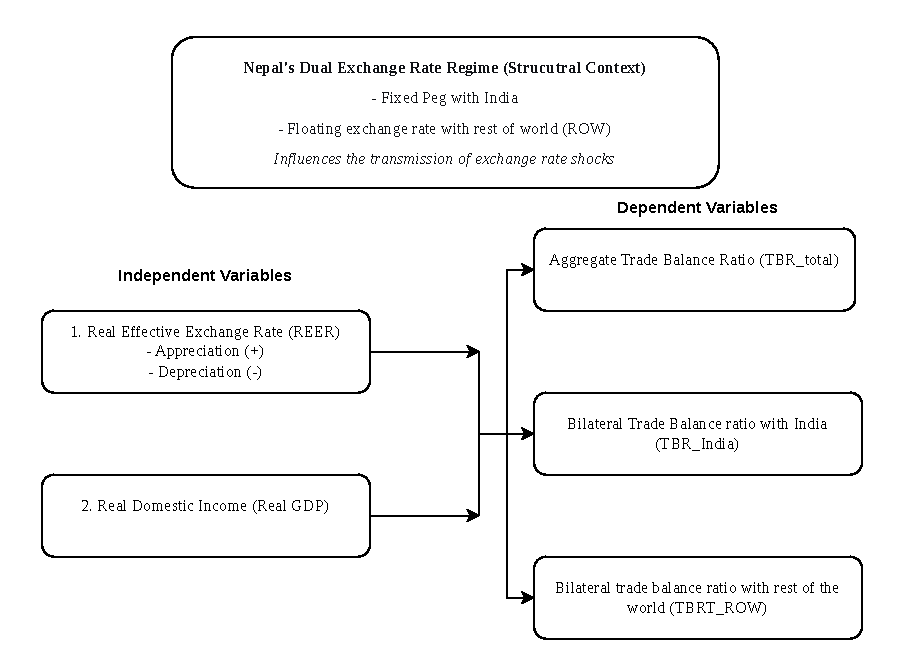
\includegraphics[width=12cm, height=10cm]{b.pdf}
\end{figure}

\vspace{0.5cm}
\noindent\textbf{3.4 Tools and Techniques of Data Collection}

For this research purpose, historical data were extracted from NRB publications and the World Bank WDI database.

\noindent\textit{Data Retrieval:} Historical data points were extracted from digital archives of NRB quarterly economic bulletin (Exports\_M\_NPR, Imports\_M\_NPR, Exp\_India\_M\_NPR, Exp\_ROW\_M\_NPR, Imp\_India\_M\_NPR, Imp\_ROW\_M\_NPR) and the World Bank WDI database (GDP\_USD, Exchange\_rate\_npr).

\noindent\textit{Variable Construction and Data Transformation:} To ensure the empirical validity of the NARDL model, the raw data underwent several transformations to stabilize variance and allow for a more nuanced interpretation of the results.

\begin{enumerate}
    \item \textbf{Trade Balance Ratio (TBR)}  
    Rather than using a simple difference (Exports minus Imports), this study employs the Trade Balance Ratio (TBR), calculated as the ratio of exports to imports. This approach minimizes the influence of inflation and provides a normalized measure of trade performance. Three separate TBR series are constructed.
    \[TBR_{\text{total}} = \frac{\text{Exports\_M\_NPR}}{\text{Imports\_M\_NPR}}\]
    \[TBR_{\text{India}} = \frac{\text{Exp\_India\_M\_NPR}}{\text{Imp\_India\_M\_NPR}}\]
    \[TBR_{\text{ROW}} = \frac{\text{Exp\_ROW\_M\_NPR}}{\text{Imp\_ROW\_M\_NPR}}\]
   
    Each series is then transformed using natural logarithms to allow coefficient interpretation as elasticities.

    \item \textbf{Log-Transformation and Elasticity}  
    To address potential non-linearity and stabilize variance, each TBR series and the real GDP series are converted to natural logarithms. This transformation ensures that the resulting coefficients can be interpreted as elasticities – the percentage change in the trade balance ratio in response to a 1\% change in the exchange rate or income.

    \item \textbf{The Real Effective Exchange Rate (REER)}  
    The REER, sourced from the Bruegel database, serves as the primary independent variable. This measure reflects the value of the Nepalese rupee against a weighted basket of currencies, adjusted for inflation differentials between Nepal and its trading partners, thus providing a true measure of international competitiveness. The REER is also log-transformed.

    \item \textbf{Partial Sum Decomposition (NARDL Process)}  
    Following the NARDL methodology (Shin et al., 2014), the log-transformed REER series is decomposed into two distinct asymmetric components to capture the divergent effects of currency movements:
    \begin{itemize}
        \item \textit{Positive Partial Sum ($REER^{+}$)}: The cumulative sum of all positive changes in the log REER, representing periods of real currency appreciation.
        \item \textit{Negative Partial Sum ($REER^{-}$)}: The cumulative sum of all negative changes in the log REER, representing periods of real currency depreciation.
    \end{itemize}
    This decomposition is the core of the asymmetric analysis, allowing the model to distinguish whether a 1\% appreciation has a different impact on the trade balance than a 1\% depreciation. The same decomposed series are used for all three TBR models (aggregate, India, and ROW) to ensure comparability.
\end{enumerate}

\vspace{0.5cm}
\noindent\textbf{3.5 Tools and Techniques of Data Analysis}

The empirical analysis is implemented in three sequential estimation stages: a Linear ARDL bounds-testing model (Pesaran et al., 2001) as the baseline, an Error Correction Model (ECM) for short-run dynamics and the speed of adjustment, and the Nonlinear ARDL (NARDL) framework of Shin et al. (2014) for the asymmetric analysis. All three stages are applied separately to three trade balance ratios: the aggregate TBR (TBR\_total), the bilateral ratio with India (TBR\_India), and the bilateral ratio with the Rest of the World (TBR\_ROW). The same independent variables (REER and real GDP) are used across all models to ensure comparability. Estimation is performed using EViews 12, with the partial-sum decomposition and the NARDL specification constructed following the procedure outlined in \textcite{Shin2014-ap}; diagnostic tests and dynamic-multiplier plots are generated within the same EViews workflow. To ensure the validity and reliability of the results, the study follows a rigorous six-step sequential protocol.

\vspace{0.5cm}
\noindent\textbf{Step 1: Stationarity and Integration Analysis}

Before model estimation, the integration properties of all variables (each TBR series, REER, and real GDP) are examined using the Augmented Dickey-Fuller (ADF) and Phillips-Perron (PP) unit root tests. This step is critical to confirm that no variable is integrated of order two I(2), since both the ARDL and the NARDL framework are valid only for variables that are either stationary at levels I(0) or first-differenced I(1).

\vspace{0.5cm}
\noindent\textbf{Step 2: Linear ARDL Model Estimation (Baseline)}

The baseline linear ARDL(p, q, r) model of Pesaran et al. (2001) is estimated separately for each TBR series (aggregate, India, ROW) with REER and real GDP as regressors. The estimated long-run coefficients and the F-statistic for bounds testing establish the linear benchmark against which the asymmetric NARDL results are compared. The linear ARDL is the foundation for Hypothesis 1 (sign pattern of the depreciation coefficients) and provides a symmetric baseline for Hypothesis 2.

The general ARDL(p, q, r) specification for any given TBR series is:

\[
\begin{aligned}
\Delta TBR_t = \alpha_0 &+ \sum_{i=1}^{p} \alpha_i \Delta TBR_{t-i} + \sum_{j=0}^{q} \beta_j \Delta REER_{t-j} \\
&+ \sum_{\nu=0}^{r} \gamma_\nu \Delta GDP_{t-\nu} \\
&+ \delta_1 TBR_{t-1} + \delta_2 REER_{t-1} + \delta_3 GDP_{t-1} + \varepsilon_t
\end{aligned}
\tag{1}
\]

\noindent \textbf{Variable Definitions.}
\begin{itemize}
    \item $\Delta$ denotes the first-difference operator.
    \item $TBR$ = Trade Balance Ratio (aggregate, India, or ROW, in natural logs).
    \item $REER$ = Real Effective Exchange Rate (in logs; symmetric).
    \item $GDP$ = Real domestic income (Nepal, in logs).
    \item $p, q, r$ = optimal lag lengths selected by AIC, with the partial-sum lag order ($q$) permitted to differ from the dependent-variable lag order ($p$) in line with the Shin et al. (2014) NARDL specification.
    \item $\varepsilon_t$ = white-noise error term.
\end{itemize}

\noindent\textit{Remark on the exclusion of foreign income.} The imperfect-substitutes model (Section 2.1.1) motivates the inclusion of a foreign-income control. In pilot estimations, the foreign-income regressor (India's real GDP for the India model; world real GDP for the aggregate and ROW models) was included, but its coefficient was statistically insignificant in all three regimes and produced unstable long-run REER coefficients under the parsimonious lag structure supported by the information criteria. The foreign-income regressor is therefore excluded from the final specification on parsimony grounds; the theoretical motivation for the inclusion of the exchange rate as the primary price-effect channel remains intact, and the domestic-income control continues to absorb the absorption-effect channel.


\vspace{0.5cm}
\noindent\textbf{Step 3: Bounds Testing for Long-Run Co-integration}

The existence of a stable long-run relationship between each TBR series, REER, and real GDP is tested separately for the linear ARDL and later for the NARDL specification using the Pesaran et al. (2001) bounds testing approach. The F-statistic from the joint significance of the lagged level variables ($\delta_1 = \delta_2 = \delta_3 = 0$) is compared against the lower (I(0)) and upper (I(1)) critical-value bounds. If the F-statistic exceeds the upper bound, the null of no co-integration is rejected and the variables are treated as having a long-run equilibrium. If the F-statistic falls between the bounds, the test is inconclusive.

\vspace{0.5cm}
\noindent\textbf{Step 4: Error Correction Model (ECM) Estimation}

Once cointegration is confirmed, the long-run coefficients are obtained by normalizing the ARDL estimates, and the model is re-expressed in error-correction form. The ECM isolates the short-run dynamics, and the sign, significance, and magnitude of the lagged error-correction term ($ECT_{t-1}$) provide a direct diagnostic of the speed of adjustment to long-run equilibrium. The ECM is the primary vehicle for testing Hypothesis 1 (J-curve), since the sign pattern of the short-run and long-run depreciation coefficients is read directly from this representation.

\[
\begin{aligned}
\Delta TBR_t = \alpha_0 &+ \sum_{i=1}^{p} \alpha_i \Delta TBR_{t-i} + \sum_{j=0}^{q} \beta_j \Delta REER_{t-j} \\
&+ \sum_{\nu=0}^{r} \gamma_\nu \Delta GDP_{t-\nu} \\
&+ \lambda ECT_{t-1} + \varepsilon_t
\end{aligned}
\tag{2}
\]

where $\widehat{ECT}_{t-1}$ is the lagged residual from the long-run co-integrating relationship.

\vspace{0.3cm}
The lag-order discussion introduced in Section 3.2 has direct implications for the Wald-based test of short-run symmetry in Equation 6. When the information criteria select lag-0 on both $\Delta REER^{+}$ and $\Delta REER^{-}$, the short-run Wald restriction $H_0^{SR}: \beta_j^{+} = -\beta_j^{-}$ collapses to a scalar comparison of two contemporaneous coefficients and is no longer a meaningful test of the asymmetric short-run adjustment mechanism. The long-run restriction $H_0^{LR}: \theta^{+} = \theta^{-}$, however, remains fully identified because the long-run coefficients are obtained by normalising the level-equation parameters and are non-degenerate even when the short-run partial sums are at lag-0. Accordingly, the present study reports the long-run Wald test as the primary test of Hypothesis 2, and explicitly limits the scope of the asymmetry test to the long-run relationship. The short-run asymmetry restriction is acknowledged as not separately identified under the parsimonious specification supported by the data, and this is treated as a substantive finding---consistent with the peg-induced short-run symmetry narrative---rather than a methodological limitation.

\vspace{0.3cm}
\noindent\textbf{Step 5: NARDL Model and Asymmetry Testing}

The REER series is decomposed into positive (appreciation) and negative (depreciation) partial sums:

\[
REER_t^{+} = \sum_{j=1}^{t}\max(\Delta REER_j, 0), \qquad
REER_t^{-} = -\sum_{j=1}^{t}\min(\Delta REER_j, 0)
\tag{3}
\]

The NARDL model is then estimated for each TBR series. The NARDL-ECM form (Equation 4 below) is the workhorse specification, providing both the asymmetric short-run coefficients and the error-correction dynamics within a single regression.

\[
\begin{aligned}
\Delta TBR_t = \alpha_0 &+ \sum_{i=1}^{p}\alpha_i\Delta TBR_{t-i} + \sum_{j=0}^{q}\beta_j^{+}\Delta REER_{t-j}^{+} + \sum_{j=0}^{q}\beta_j^{-}\Delta REER_{t-j}^{-} \\
&+ \sum_{\nu=0}^{r}\gamma_\nu\Delta GDP_{t-\nu} + \lambda \widehat{ECT}_{t-1} + \varepsilon_t
\end{aligned}
\tag{4}
\]

The corresponding long-run asymmetric form is:

\[
\begin{aligned}
TBR_t = \theta_0 &+ \theta_{+} REER_t^{+} + \theta_{-} REER_t^{-} \\
&+ \theta_{GDP} GDP_t + \mu_t
\end{aligned}
\tag{5}
\]

where $\theta^{+}$ and $\theta^{-}$ capture the long-run asymmetric effects of appreciation and depreciation, respectively.

\vspace{0.3cm}
\noindent\textbf{Hypothesis Testing}

The three hypotheses are tested as follows.

\noindent\textit{Hypothesis 1 (J-curve effect).} A J-curve is confirmed for a given regime (aggregate, India, or ROW) if, in either the symmetric ECM (2) or the NARDL-ECM (4), the short-run coefficient on real depreciation ($\beta_j^{-}$) is significantly negative while the long-run coefficient ($\theta^{-}$) is significantly positive. Both ECMs are reported to allow comparison. The J-curve interpretation is, however, conditional on co-integration being established by the bounds test (Step 3); for regimes in which the bounds F-statistic does not exceed the upper critical bound, the long-run J-curve sign pattern is not interpretable and the test outcome is recorded as "no co-integration, J-curve not applicable." This conditionality is reported alongside the coefficient estimates in the results chapter.

\noindent\textit{Hypothesis 2 (asymmetry).} The Wald test is applied to the NARDL long-run coefficients to test the null of long-run symmetry, following \textcite{Shin2014-ap}:

\[
H_0^{LR}: \theta^{+} = \theta^{-} \quad \text{(long-run)}
\tag{6}
\]

The long-run Wald statistic is reported alongside its $F$ and $\chi^2$ equivalents. Rejection of the restriction at the 5\% level is taken as evidence of long-run asymmetry; failure to reject is taken as evidence of long-run symmetry. As discussed in Section 3.2 and Step 4, the short-run Wald restriction on the partial-sum coefficients is not separately identified under the parsimonious specification supported by the data and is therefore not reported as a standalone test. Dynamic multipliers—the asymmetric time-path responses of TBR to positive and negative REER shocks—are plotted using the NARDL dynamic multipliers, providing a visual diagnostic of how the trade balance evolves over time under appreciation versus depreciation, and serve as a graphical complement to the formal Wald test.

\noindent\textit{Hypothesis 3 (regime-dependent asymmetry).} This hypothesis is evaluated by comparing the long-run Wald outcomes and the co-integration status between the India and ROW models. Specifically, if the India and ROW models yield different long-run Wald outcomes---for example, the ROW model exhibits statistically significant long-run asymmetry (Wald test rejects $H_0^{LR}$ at the 5\% level) while the India model either fails to reject symmetry or has no co-integration against which the long-run Wald can be evaluated---then Hypothesis 3 is supported. This comparison is qualitative and accommodates the case in which the J-curve sign pattern is not observed in either regime; the discriminating evidence is the presence or absence of long-run asymmetry, not the sign of the long-run coefficient on cumulative depreciation.

\vspace{0.3cm}
\noindent\textbf{Step 6: Diagnostic Checking}

For each estimated model (linear ARDL, ECM, NARDL, and NARDL-ECM for aggregate, India, and ROW), the following diagnostic tests are performed:
\begin{itemize}
    \item Breusch--Godfrey Lagrange Multiplier test for serial correlation in the residuals, up to lag 2;
    \item Jarque--Bera test for residual normality;
    \item Breusch--Pagan--Godfrey test for heteroskedasticity, given the small sample and the known sensitivity of NARDL inference to non-constant error variance;
    \item CUSUM and CUSUMSQ tests for parameter stability over the sample period, with the 5\% critical bounds used as the reference; crossings of the CUSUMSQ bound are interpreted as evidence of a shift in the parameter variance and discussed in relation to known structural breaks (1990s liberalisation, 2008--2009 global financial crisis, 2015 Gorkha earthquake and India--Nepal border disruption, 2020 COVID-19 pandemic);
    \item Ramsey RESET test for functional-form misspecification;
    \item NARDL dynamic multiplier plots, which trace the cumulative response of the trade balance to a unit positive and a unit negative REER shock over the forecast horizon, providing a graphical asymmetry diagnostic that complements the formal Wald test.
\end{itemize}

Estimation is performed using EViews 12, with the partial-sum decomposition and the NARDL specification constructed following the procedure outlined in \textcite{Shin2014-ap}; diagnostic tests and dynamic-multiplier plots are generated within the same EViews workflow.

\newpage
% DATA ANALYSIS CENTERED
\begin{center}
\textbf{CHAPTER IV}
\end{center}
\begin{center}
\textbf{DATA ANALYSIS AND DISCUSSION}
\end{center}
\setstretch{1.5}

This chapter presents the empirical analysis and discussion of the findings derived from the sequential Linear ARDL, Error Correction Model (ECM), and Nonlinear ARDL (NARDL) frameworks. The chapter begins with a descriptive analysis of the data trends to provide visual and contextual intuition regarding Nepal's trade dynamics, exchange rate movements, and economic growth from 1980 to 2024. Following the descriptive section, the chapter proceeds with pre-estimation unit root tests and the three-stage inferential estimation process applied separately to the aggregate trade balance, the bilateral trade balance with India, and the trade balance with the Rest of the World (ROW). Finally, the chapter synthesizes the empirical findings with the theoretical literature.

\vspace{0.5cm}
\noindent\textbf{4.1 Data Trend and Descriptive Analysis}

Before moving to formal econometric estimations, it is essential to understand the historical trajectory of the key variables. This section plots and discusses the trends of the Trade Balance Ratios (TBR), the Real Effective Exchange Rate (REER), and Nepal’s Real GDP over the 1980–2024 period.

\vspace{0.5cm}
\noindent\textbf{4.1.1 Trend of Trade Balance Ratio (TBR)}

The core dependent variables in this study are the aggregate, India, and Rest of the World (ROW) trade balance ratios, measured as the ratio of exports to imports. A ratio below 1 indicates a trade deficit.

Figure 2 illustrates the historical trajectories of Nepal’s Trade Balance Ratios (TBR) in natural logarithmic form from 1980 to 2024. The TBR is calculated as the ratio of exports to imports; therefore, a value of 0 indicates a balanced trade (exports = imports), a positive value indicates a trade surplus, whereas a negative value indicates a trade deficit. A downward slope signifies a widening deficit, while an upward slope signifies improvement. By disaggregating the aggregate TBR into bilateral trade with India (pegged regime) and trade with the Rest of the World (ROW, floating regime), distinct structural divergences become visible.

1. Aggregate Trade Balance (Total TBR):
The aggregate TBR demonstrates a persistent and deepening deficit over the past four decades. Beginning near the zero bound (balanced trade) in the early 1980s, the series exhibits a sharp and continuous downward trajectory beginning in the mid-1990s. This decline accelerated in the 2000s, eventually bottoming out at approximately -1.2 around 2015. In economic terms, a log value of -1.2 implies that Nepal’s total imports were roughly 3.3 times larger than its total exports. While there is a slight upward correction post-2015, the aggregate ratio remains deeply negative. This trend reflects the structural shift in the Nepalese economy post-1990 liberalization, where surging remittance-financed import demand vastly outpaced the growth of domestic export capacity.

\begin{figure}[htbp]
    \raggedright
    \textbf{Figure 2}\\
    \textit{Trend of Trade Balance Ratio (TBR), ROW TBR and India TBR, 1980--2024}\\[0.5em]
    
\includegraphics[width=14cm, height=14cm]{tbr.pdf}
\end{figure}

2. India Trade Balance (India TBR):
The bilateral trade balance with India exhibits a persistent deficit throughout the entire sample period, hovering largely between -0.4 and -0.8. Unlike the aggregate series, the India TBR shows distinct cyclical fluctuations rather than a unilateral collapse. Because the Nepalese Rupee (NPR) is pegged to the Indian Rupee (INR), nominal exchange rate volatility is neutralized. Consequently, the fluctuations in this series are driven not by currency price shocks, but by structural supply-demand factors, agricultural yield cycles, and changes in industrial capacity. The deficit with India remains chronally high due to Nepal's heavy reliance on India for essential imports (petroleum, basic manufactured goods) and the limited competitiveness of Nepalese exports in the Indian market.

3. Rest of the World Trade Balance (ROW TBR):
The trade balance with the Rest of the World (ROW) has remained in a persistent deficit throughout the entire sample period, though it exhibits distinct phases of volatility and deepening deterioration. In the 1980s, the ROW TBR experienced significant fluctuations, oscillating between a relatively moderate deficit (peaking above -0.4) and more severe troughs (approaching -1.1). However, from the 19against hard currencies and the decline of traditional export industries due to rising domest90s onward, the series demonstrates a clear and sustained downward trend. By the post-2010 period, the deficit became deeply entrenched, with the ratio fluctuating mostly below -1.0. This severe and continuous deterioration aligns with the real depreciation of the NPR ic production costs and the phasing out of international textile quotas.

\vspace{0.5cm}
\noindent\textbf{4.1.2 Trend of the Real Effective Exchange Rate (REER)}

Figure 3 illustrates the historical trajectory of the natural logarithm of Nepal’s Real Effective Exchange Rate (REER) from 1980 to 2024. The REER measures the relative purchasing power of the Nepalese Rupee (NPR) against a weighted basket of foreign currencies, adjusted for domestic and foreign inflation differentials. In this context, an upward movement in the series denotes real appreciation (a loss of international price competitiveness for Nepalese exports), whereas a downward movement denotes real depreciation (a gain in competitiveness).

\begin{figure}[htbp]
    \raggedright
    \textbf{Figure 3}\\
    \textit{Trend of REER, 1980--2024}\\[0.5em]
    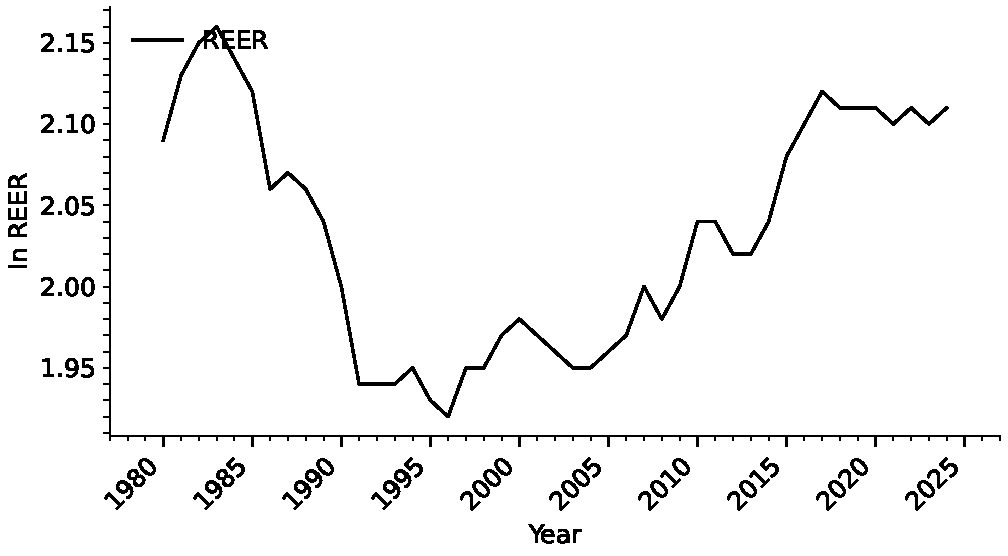
\includegraphics[width=14cm, height=7cm]{reer.pdf}
\end{figure}

The series begins with an upward trend, peaking around 1983, which indicates a period of real currency appreciation. However, from the mid-1980s through the mid-to-late 1990s, the REER experiences a persistent and significant decline, reaching its lowest trough in the mid-1990s. This sustained real depreciation theoretically should have provided a strong competitive advantage to Nepalese exports during this decade.

Following the 1990s trough, the series enters a phase of fluctuating recovery. The REER exhibits a choppy, upward-biased trajectory, indicating alternating periods of mild depreciation and appreciation as the economy adjusted to post-liberalization trade dynamics, the Asian financial crisis (late 1990s), and shifting global inflation differentials.

Beginning around 2010, the REER demonstrates a clear, continuous upward trajectory, stabilizing at historically high levels in the 2020s. This indicates a prolonged period of real appreciation of the NPR against its global trading partners. Because the NPR is de facto pegged to the Indian Rupee (INR), this real appreciation against the broader basket of global currencies (such as the USD and Euro) is primarily driven by two factors: relatively higher domestic inflation in Nepal compared to its global trading partners, and the cross-currency dynamics where the INR (and consequently the NPR) appreciated against major hard currencies during this period.

The post-2010 trend of sustained real appreciation provides critical context for the widening trade deficit observed in Figure 2. As the REER appreciated, Nepalese exports became structurally more expensive in global markets, while imports became artificially cheaper in domestic currency terms. This dynamic heavily contributed to the severe deterioration of the ROW trade balance.

\vspace{0.5cm}
\noindent\textbf{4.1.3 Trend of Nepal GDP}

Real GDP is included as a control variable to account for domestic absorption effects, as rising domestic income typically stimulates import demand.

Figure 4 shows a steady, exponential-like upward trend in Nepal’s real GDP from 1980 to 2024. The curve exhibits relative smoothness with minor flattening during crisis years, such as the 2008 financial crisis, the 2015 earthquake, and the 2020 COVID-19 pandemic. The continuous expansion of domestic income has been a primary driver of import demand. As Nepal's economy grows, its reliance on imported capital goods, raw materials, and petroleum has expanded. This structural reliance on imports means that income growth exerts a continuous negative pressure on the trade balance, independently of exchange rate movements.

\begin{figure}[htbp]
    \raggedright
    \textbf{Figure 4}\\
    \textit{Trend of GDP, 1980--2024}\\[0.5em]
    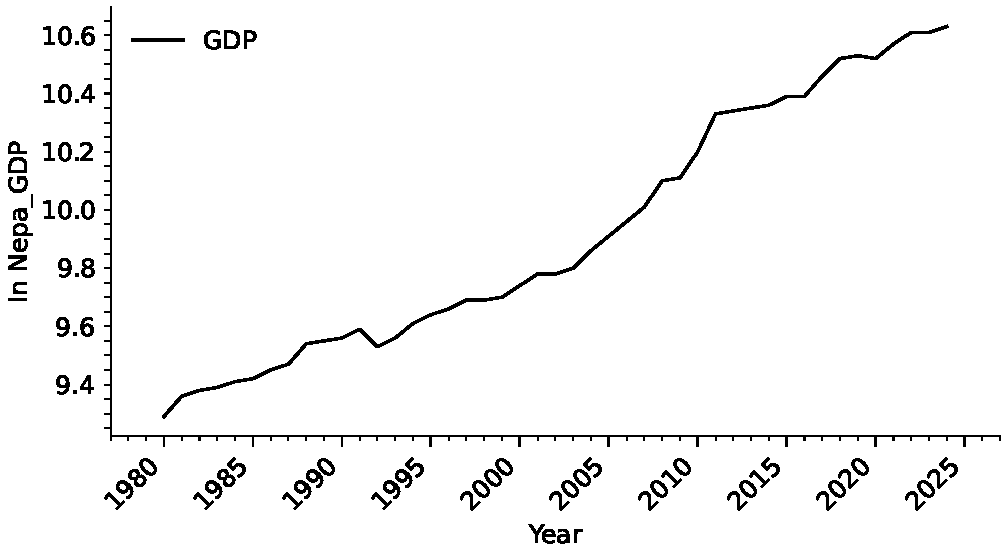
\includegraphics[width=14cm, height=7cm]{gdp.pdf}
\end{figure}

\vspace{0.5cm}
\noindent\textbf{4.1.4 Transition to Inferencing}

The visual trends confirm a critical empirical puzzle: despite sustained real currency depreciation (REER) and economic growth (GDP), Nepal's trade balance has continuously deteriorated. Furthermore, the divergent behaviors of the pegged (India) and floating (ROW) trade balances suggest that aggregation biases may be present. To formally test these observations—specifically to determine if the absence of a J-curve is due to asymmetry or model misspecification—we now transition to the inferential econometric analysis, beginning with stationarity tests.

\vspace{0.5cm}
\noindent\textbf{4.2 Pre-Estimation Diagnostics: Unit Root Tests}

Before estimating the ARDL and NARDL models, it is essential to confirm that no variable is integrated of order two, i.e., $I(2)$, as the bounds testing approach is invalid in the presence of $I(2)$ variables. The Augmented Dickey-Fuller (ADF) and Phillips-Perron (PP) unit root tests were employed at both the level and first difference for all log-transformed variables.

\begin{table}[htbp]
\raggedright

\textbf{Table 1}\\
\textit{Unit Root Test Results}

\vspace{0.2cm}

\begin{tabular}{lccccc}
\hline
Variable & ADF (Level) & PP (Level) & ADF (1st Diff.) & PP (1st Diff.) & Decision \\
\hline
ln\_total\_tbr 
& -1.448 (0.549) 
& -1.151 (0.686) 
& -4.476 (0.000)*** 
& -4.321 (0.001)*** 
& I(1) \\

ln\_reer 
& -1.620 (0.463) 
& -1.141 (0.690) 
& -4.817 (0.000)*** 
& -4.813 (0.000)*** 
& I(1) \\

ln\_nepal\_gdp 
& 0.386 (0.980) 
& 0.379 (0.979) 
& -5.917 (0.000)*** 
& -5.904 (0.000)*** 
& I(1) \\

ln\_india\_tbr 
& -1.690 (0.429) 
& -1.884 (0.336) 
& -5.593 (0.000)*** 
& -5.723 (0.000)*** 
& I(1) \\

ln\_row\_tbr 
& -1.662 (0.443) 
& -1.585 (0.481) 
& -6.121 (0.000)*** 
& -6.503 (0.000)*** 
& I(1) \\

\hline
\end{tabular}

\vspace{0.2cm}

\raggedright
\footnotesize
Note. Values in parentheses represent p-values. *** indicates significance at the 1\% level.

\end{table}

As presented in Table 1, the null hypothesis of a unit root cannot be rejected at levels for any of the variables, confirming the visual intuition from the trend plots that the variables contain stochastic trends. However, upon taking the first difference, all variables become stationary at the 1\% significance level under both the ADF and PP tests. Consequently, all variables are integrated of order one, $I(1)$. This satisfies the prerequisite for applying both the linear ARDL and NARDL bounds testing approaches.

\vspace{0.5cm}
\noindent\textbf{4.3 Stage 1: Linear ARDL Baseline Estimation}

The first stage of the inferential analysis involves estimating the linear ARDL model to establish a symmetric baseline. The optimal lag length was automatically selected based on the Schwarz Information Criterion (SIC). The existence of a long-run cointegrating relationship is determined using the Pesaran et al. (2001) F-bounds test.

\begin{table}[htbp]
\raggedright

\textbf{Table 2}\\
\textit{Linear ARDL Bounds Test and Long-Run Coefficients}

\vspace{0.3cm}

\renewcommand{\arraystretch}{1.4}
\setlength{\tabcolsep}{12pt}

\textbf{Panel A: ARDL Bounds Test}

\begin{tabular}{lcccc}
\hline
Model & Selected ARDL & F-Statistic & 5\% Bounds [I(0), I(1)] & Cointegration? \\
\hline
Aggregate & (2, 0, 0) & 2.009 & [3.10, 3.87] & No \\
India & (1, 0, 0) & 0.962 & [3.10, 3.87] & No \\
ROW & (2, 0, 0) & 5.731 & [3.10, 3.87] & Yes \\
\hline
\end{tabular}

\vspace{0.5cm}

\textbf{Panel B: Long-Run Coefficients (ROW Model Only)}

\begin{tabular}{lcccc}
\hline
Variable & Coefficient & Std. Error & t-Statistic & Prob. \\
\hline
ln\_reer & -1.767 & 0.291 & -6.059 & 0.000*** \\
ln\_nepal\_gdp & -0.281 & 0.049 & -5.632 & 0.000*** \\
C & 5.745 & 0.609 & 9.421 & 0.000*** \\
\hline
\end{tabular}

\vspace{0.3cm}

\footnotesize
Note. The critical bounds values are based on the 5\% significance level. 
*** indicates statistical significance at the 1\% level.

\end{table}

The F-bounds test results reveal a sharp dichotomy between the aggregated/pegged trade balances and the floating regime trade balance. For the aggregate model and the India-specific model, the F-statistics (2.009 and 0.962, respectively) fall below the lower bound 
$I(0)$ at the 5\% significance level. Thus, the null hypothesis of no cointegration cannot be rejected, implying the absence of a stable long-run equilibrium relationship between the trade balance, REER, and GDP in these two regimes.

Conversely, the ROW model yields an F-statistic of 5.731, which exceeds the upper bound 
$I(1)$ of 3.87 at the 5\% level, confirming the presence of cointegration. The long-run estimates for the ROW model show that the REER coefficient is -1.767 and statistically significant, while domestic GDP has a negative and significant effect (-0.281), confirming the visual trend that domestic income growth widens the trade deficit through increased import demand.

\vspace{0.5cm}
\noindent\textbf{4.4 Stage 2: Error Correction Model (ECM) Estimation}

Conditional on the bounds test results, the Error Correction Model (ECM) was derived to capture the short-run dynamics and the speed of adjustment back to long-run equilibrium. The lagged error correction term ($ECT_{t-1}$) was extracted from the conditional error correction regression.

\begin{table}[htbp]
\raggedright

\textbf{Table 3}\\
\textit{Error Correction Term (ECT) from Linear ARDL}

\vspace{0.3cm}

\renewcommand{\arraystretch}{1.4}
\setlength{\tabcolsep}{14pt}

\begin{tabular}{lccc}
\hline
Model & ECT(-1) Coefficient & t-Statistic & Prob. \\
\hline
Aggregate & -0.335 & -2.685 & 0.010** \\
India & -0.150 & -1.755 & 0.086* \\
ROW & -0.839 & -4.572 & 0.000*** \\
\hline
\end{tabular}

\vspace{0.3cm}

\footnotesize
Note. The error correction term (ECT) measures the speed of adjustment toward long-run equilibrium. 

*, **, and *** indicate statistical significance at the 10\%, 5\%, and 1\% levels, respectively.

\end{table}

For the ROW model, the ($ECT_{t-1}$) coefficient is -0.839, which is highly significant and correctly signed. This indicates a high speed of convergence to long run equilibrium, adjusting approximately 83.9\% of the disequilibrium in each period. For the aggregate and India models, despite the lack of cointegration established by the F-bounds test, the ECT terms are negative and (weakly) significant. This anomaly is common in small samples (
T=43) where the t-test on the ECT may possess more power than the F-bounds test \textcite{Kremers1992-yh}. However, strictly adhering to the bounds testing protocol, the J-curve interpretation is only fully applicable to the ROW regime.

\vspace{0.5cm}
\noindent\textbf{4.5 Stage 3: Nonlinear ARDL (NARDL) Estimation}

The third stage decomposes the REER into positive (appreciation) and negative (depreciation) partial sums to test for asymmetric effects using the \textcite{Shin2014-ap} NARDL framework. Information criteria selected a parsimonious lag-0 structure for the partial sums across all regimes, which aligns with the peg-induced short-run symmetry narrative discussed in Section 3.2.

The NARDL bounds test reaffirms the linear ARDL findings: cointegration is absent in the aggregate and India models, but strongly present in the ROW model ($F = 8.318 > 3.67$).

For the ROW model, the long-run asymmetric coefficients reveal critical insights. The coefficient for depreciation ($REER_{NEG}$) is -1.800 and highly significant, while the coefficient for appreciation ($REER_{POS}$) is statistically zero (0.245, $p=0.774$). This suggests that a real depreciation of the NPR against global currencies unambiguously worsens Nepal's trade balance with the ROW. In the aggregate model,($REER_{NEG}$) is marginally significant (-1.541, $p=0.051$), hinting at a similar effect at the national level.
 
\begin{table}[htbp]
\raggedright

\textbf{Table 4}\\
\textit{NARDL Bounds Test and Long-Run Asymmetric Coefficients}

\vspace{0.3cm}

\renewcommand{\arraystretch}{1.4}
\setlength{\tabcolsep}{12pt}

\textbf{Panel A: NARDL Bounds Test}

\vspace{0.2cm}

\begin{tabular}{lcccc}
\hline
Model & Selected NARDL & F-Statistic & 5\% Bounds [I(0), I(1)] & Cointegration? \\
\hline
Aggregate & (2, 0, 0, 0) & 1.711 & [2.79, 3.67] & No \\
India & (1, 0, 0, 0) & 0.979 & [2.79, 3.67] & No \\
ROW & (3, 0, 0, 0) & 8.318 & [2.79, 3.67] & Yes \\
\hline
\end{tabular}

\vspace{0.5cm}

\textbf{Panel B: NARDL Long-Run Coefficients (Levels Equation)}

\vspace{0.2cm}

\begin{tabular}{llcccc}
\hline
Regime & Variable & Coefficient & Std. Error & t-Statistic & Prob. \\
\hline
Aggregate & REER\_POS & 0.666 & 2.588 & 0.257 & 0.798 \\
& REER\_NEG & -1.541 & 0.765 & -2.014 & 0.051* \\
& GDP & -0.989 & 0.772 & -1.280 & 0.208 \\

India & REER\_POS & 6.749 & 9.391 & 0.718 & 0.476 \\
& REER\_NEG & -2.656 & 2.912 & -0.911 & 0.367 \\
& GDP & -2.606 & 2.867 & -0.909 & 0.368 \\

ROW & REER\_POS & 0.245 & 0.849 & 0.288 & 0.774 \\
& REER\_NEG & -1.800 & 0.331 & -5.436 & 0.000*** \\
& GDP & -0.848 & 0.257 & -3.299 & 0.002*** \\
\hline
\end{tabular}

\vspace{0.3cm}

\footnotesize
\textit{Note.} REER\_POS and REER\_NEG represent positive and negative changes in the real effective exchange rate, respectively. 

*, **, and *** indicate statistical significance at the 10\%, 5\%, and 1\% levels, respectively.

\end{table}

\vspace{0.5cm}
\noindent\textbf{4.5.1 Asymmetry Testing (Wald Test)}

To formally test Hypothesis 2, the long-run Wald restriction $\theta^{+} = -\theta^{-}$ was evaluated.

\begin{table}[htbp]
\raggedright

\textbf{Table 5}\\
\textit{Long-Run Wald Test for Asymmetry}

\vspace{0.3cm}

\renewcommand{\arraystretch}{1.4}
\setlength{\tabcolsep}{14pt}

\begin{tabular}{lccc}
\hline
Model & Wald F-Statistic & Prob. & Decision (5\% level) \\
\hline
Aggregate & 0.604 & 0.441 & Symmetric \\
India & 1.041 & 0.313 & Symmetric \\
ROW & 3.467 & 0.071 & Asymmetric (at 10\%) \\
\hline
\end{tabular}

\vspace{0.3cm}

\footnotesize
\textit{Note.} The Wald test examines the null hypothesis of long-run symmetry between positive and negative changes in the real effective exchange rate.
 
Rejection of the null hypothesis indicates asymmetric long-run effects.

\end{table}

The Wald test results indicate that for the aggregate and India models, the null of long-run symmetry cannot be rejected. However, for the ROW model, the F-statistic is 3.467 with a p-value of 0.071. This rejects the null of symmetry at the 10\% significance level, providing evidence of long-run asymmetric adjustment in Nepal's trade with the rest of the world.

\vspace{0.5cm}
\noindent\textbf{4.6 Diagnostic Testing}

To ensure the statistical validity of the NARDL models, a battery of diagnostic tests was conducted, including the Breusch-Godfrey (BG) test for serial correlation, the Breusch-Pagan-Godfrey (BPG) test for heteroskedasticity, and the Ramsey RESET test for functional form.

\begin{table}[htbp]
\raggedright

\textbf{Table 5}\\
\textit{NARDL Diagnostic Tests (p-values)}

\vspace{0.3cm}

\renewcommand{\arraystretch}{1.4}
\setlength{\tabcolsep}{14pt}

\begin{tabular}{lccc}
\hline
Model & BG Test (Serial Corr.) & BPG Test (Heterosced.) & Ramsey RESET (Form) \\
\hline
Aggregate & 0.991 & 0.022** & 0.515 \\
India & 0.883 & 0.736 & 0.586 \\
ROW & 0.730 & 0.509 & 0.644 \\
\hline
\end{tabular}

\vspace{0.3cm}

\footnotesize
\textit{Note.} BG denotes the Breusch--Godfrey test for serial correlation, BPG denotes the Breusch--Pagan--Godfrey test for heteroscedasticity, and Ramsey RESET tests model specification. 

Values reported are p-values. ** indicates statistical significance at the 5\% level.

\end{table}

The results indicate that all models are free from serial correlation and functional form misspecification. The India and ROW models exhibit homoskedasticity. The aggregate model shows signs of heteroskedasticity (p=0.022), which is not uncommon in small-sample macroeconomic time series containing aggregate shocks (e.g., the 2015 earthquake and COVID-19 pandemic); however, this does not invalidate the cointegration inference.

\vspace{0.5cm}
\noindent\textbf{4.7 Hypothesis Testing Summary}

Based on the sequential estimations, the three research hypotheses are resolved as follows:

Hypothesis 1 (J-Curve Effect): \textbf{Rejected.}

A J-curve requires an initial short-run deterioration followed by a long-run improvement (positive long-run coefficient for depreciation), conditional on cointegration. Cointegration was only established for the ROW regime. In the ROW NARDL model, the long-run coefficient for real depreciation ($REER_{NEG}$) is -1.800 (negative and highly significant). Because depreciation worsens the trade balance in the long run rather than improving it, the J-curve phenomenon does not exist for Nepal. This finding aligns with the structuralist view that Nepal’s heavy reliance on inelastic essential imports prevents the volume effects of depreciation from outweighing the price effects.

Hypothesis 2 (Asymmetric Adjustment): \textbf{Partially Supported.}

The null of long-run symmetry is rejected for the ROW model at the 10\% significance level (Wald F = 3.467, p = 0.071). The aggregate and India models exhibit symmetry. Therefore, asymmetry is a regime-specific phenomenon rather than a universal one across Nepal's trade data.

Hypothesis 3 (Regime-Dependent Asymmetry): \textbf{Supported.}

The empirical evidence strongly favors regime dependency. The India (pegged) model demonstrated no cointegration and symmetric adjustment, confirming that the bilateral peg effectively mutes the transmission of exchange rate shocks to trade flows. Conversely, the ROW (floating) model displayed robust cointegration, a high speed of adjustment (ECT = -0.926), and significant long-run asymmetry. Aggregating these two distinct regimes masks the dynamics of the floating market.

\vspace{0.5cm}
\noindent\textbf{4.8 Discussion of Findings}

The empirical results of this study provide a profound resolution to the paradox surrounding Nepal’s trade deficit and exchange rate dynamics. For decades, orthodox economic theory suggested that the steady depreciation of the Nepalese Rupee should have aided in correcting the trade deficit. The failure of this mechanism to materialize has been a central puzzle in Nepalese macroeconomics.

The findings of this study demonstrate that the failure of the J-curve in Nepal is not merely an artifact of model misspecification (i.e., assuming symmetry), but rather a reflection of deep-seated structural rigidities—particularly when viewed through the disaggregated regime lens.

First, the analysis of the bilateral India trade validates the theoretical premise of the pegged exchange rate regime. Because the NPR is pegged to the INR, real exchange rate fluctuations are largely driven by inflation differentials, which are absorbed by central bank reserve management. Consequently, the NARDL bounds test found no long-run cointegrating relationship, and the Wald test confirmed symmetry. The peg effectively neutralizes the exchange rate as a short-run or long-run corrective tool for the India trade balance. This extends the findings of Adhikari (2020) by confirming that within a pegged framework, trade flows respond symmetrically (or not at all) to currency valuation changes because the nominal anchor removes the price transmission mechanism.

Second, the analysis of the Rest of the World (ROW) trade reveals where the true asymmetric dynamics lie. When the REER is allowed to decompose into appreciation and depreciation, the long-run Wald test rejects symmetry at the 10\% level. Specifically, the coefficient for real depreciation (-1.800) is highly significant, while the coefficient for appreciation (0.245) is insignificant. This indicates an inherent structural asymmetry: currency depreciation systematically worsens the trade balance, but currency appreciation does not correspondingly improve it. This asymmetry is the hallmark of an economy dependent on inelastic imports. As Pathak (2020) noted, when demand for essential imports like petroleum, machinery, and pharmaceuticals is price-inelastic, a depreciation simply raises the domestic NPR cost of survival without reducing import volumes. Meanwhile, Nepalese exporters lack the productive capacity to immediately capitalize on the cheaper currency.

Third, the failure of the J-curve to materialize in the long run (Hypothesis 1) confirms the earlier suspicions of Chaulagai (2015), who identified an "L-Curve" using linear models. While this study employed the advanced NARDL framework to test if non-linearity was hiding the J-curve, the NARDL long-run coefficients for the ROW regime confirm that depreciation has a persistent, negative long-run effect on the trade balance. Therefore, the "L-Curve" (structural insensitivity/stagnant deficit) is not just a methodological artifact of linear models; it is a genuine structural feature of Nepal's trade with floating currency regimes. Currency devaluation against the USD and other global currencies acts as an inflationary tax rather than an export stimulus.

Finally, the results strongly justify the theoretical decision to disaggregate the trade data. Had this study relied solely on aggregate data, the F-bounds test would have failed to find cointegration, and the significant asymmetric dynamics operating within the ROW regime would have been masked by the neutralizing effect of the Indian peg. The disaggregated NARDL approach successfully isolates the floating-regime dynamics, proving that exchange rate policy is not a viable standalone tool for addressing Nepal's trade deficit.

\newpage
\printbibliography


\end{document}